\documentclass[a4paper, 11pt]{article}

\usepackage[utf8]{inputenc}
\usepackage{verbatim}
\usepackage{moreverb}
\usepackage[english]{babel}
%\usepackage{english}
\usepackage[T1]{fontenc}
\usepackage{lmodern}
\usepackage{graphicx}
\usepackage{fancyhdr}
\usepackage{listings} 
\usepackage{lastpage}
\usepackage[top=3cm, bottom=3cm, left=2cm, right=2cm]{geometry}
\usepackage{color}
\usepackage{xcolor}
%font change
\renewcommand{\familydefault}{\sfdefault}

\newcommand{\HRule}{\rule{\linewidth}{0.5mm}}
\newcommand{\nl}{\\[0.1cm]}
\newcommand{\s}{\vspace{0.3cm}}
\newcommand{\smore}{\vspace{0.6cm}}

\usepackage{caption}
\DeclareCaptionFont{white}{\color{white}}
\DeclareCaptionFormat{listing}{\colorbox{gray}{\parbox{\textwidth}{#1#2#3}}}
\captionsetup[lstlisting]{format=listing,labelfont=white,textfont=white}

\lstset{frame=single}

\lstdefinelanguage{popc}{%
   morekeywords={%
   %od
      od, url, power, @, 100, 80, machine, POPString, search
  },
  sensitive=true,
  morestring=[b]',
}

\addto\captionsenglish{%
  \renewcommand{\listfigurename}{}%
	\renewcommand\refname{}
}



%Header and footer 
\pagestyle{fancy}
\fancyhead{}
\fancyfoot{}

%Header definition
\renewcommand{\headrulewidth}{0.5pt}
\lhead{ViSaG : Virtual Safe GRID}
\rhead{POP-C++ over SSH Tunnel}

%Footer definition
\renewcommand{\footrulewidth}{0.5pt}
\cfoot{\today}
\lfoot{Clément Valentin}
\rfoot{Page \thepage ~on \pageref{LastPage}}

%remove indent for paragraph
\parindent0ex 

%\setlength{\parskip2ex}








%\pagebreak



\begin{document}

% TITLE INFORMATION

\begin{titlepage}
 
\begin{center}

\includegraphics[scale=0.3]{logo_eif.png}\\[1.5cm]
\textsc{\LARGE ViSaG - Virtual Safe GRID}\\[1.5cm]


\includegraphics[scale=0.3]{pic/logo_pop.png}\\[2cm]


\HRule \\[1cm]
{ \huge \bfseries POP-C++ Virtual-Secure (VS)}\\[0.5cm]
\textsc{\LARGE POP-C++ User and Installation manual : add-on}\\[1cm]
 
\HRule \\[5cm]
 
% Author and supervisor
\begin{minipage}{0.4\textwidth}
\begin{flushleft} \large
\textbf{Author:}\\
Valentin Clément
\end{flushleft}
\end{minipage}
\begin{minipage}{0.4\textwidth}
\begin{flushright} \large
\textbf{Date:} \today \\

\textbf{Revision:} 1.0
\end{flushright}
\end{minipage}
 
\vfill
  
\end{center}
 
\end{titlepage}

%\newpage \thispagestyle{empty} \mbox{}\newpage



\tableofcontents
\pagebreak
\section{Introduction}
ViSaG is a project to enhance the security in a computing grid infrastructure. Under this project, the EIA-FR is in charge of the security implementation in the middle-ware POP-C++. This document explains the different mechanisms to implement inside POP-C++ to use a secure connection over SSH. This document is structured as follows : 
\begin{itemize}
\item The following chapter aims to explain why we choose the SSH tunnelling to implement a secured version of POP-C++.
\item The third chapter presents some alternatives to the SSH tunnelling.
\item The fourth chapter explains the principles of the SSH tunnelling.
\item The fifth chapter is a review of the current situation in POP-C++.
\item The sixth chapter explains the key exchange process choose for POP-C++.
\item The seventh chapter describes all the modifications made to POP-C++ to be able to use the SSH tunnelling.
\item The eighth chapter gives some future possible improvements. 
\item The ninth chapter gives to the end user the major changes that comes with the new version of POP-C++.
\item The tenth chapter is a review of two test scenarios. 
\item The eleventh chapter describes the current known issues. 
\item The last chapter concludes this report. 
\end{itemize}


%-- MOTIVATIONS
\section{Motivations}
\textit{"Why do we choose SSH tunnelling with public keys to implement the security inside the POP-C++ middle-ware ?"}\s

Due to its architecture, a parallel object executed on a node can be contacted on different ports which represent the different protocol implemented for POP-C++. A single node can execute more than one parallel object at the same time. The ports on which the parallel objects will be contacted are not defined before the launching of the application.\s

We needed a security solution that involve the less manipulations on firewalls or existing security installations. The SSH tunnelling provide the SSH security level and need only a single port opened. 


%-- ALTERNATIVES
\pagebreak
\section{Alternatives}
In this chapter, we just summarize some approaches that we have thought about before the implementation. In the future, it could also be implemented inside POP-C++. 

\subsection{TLS(SSL) Combox}
The architecture of POP-C++ let the developer the choice to implement any protocol as a "combox". TLS could be implemented as a combox but there would be a drawback. With TLS, we need to open a lot of ports on firewall and on nodes to let the application execution succeed. In fact, each object running on a node will create its own TLS Server to receive the incoming connections. If we have 20 parallel objects executing on a node, we will need to open 20 ports to let the incoming connections succeed. Due to this, we leave this approach on the side for the moment.

\subsection{SSH with username/password authentication}
A variant of SSH tunnelling using public keys is the username/password authentication. This method could be a little bit less secure because every node executing a parallel object of the application must be initialized with the same username/password pair. On the other side, this method could reduce the traffic generated by the keys exchange. In fact, the interface just need to provide the pair username/password to create the tunnel instead of transfer its key to the node executing the parallel object.


\pagebreak
%-- SSH TUNNELING
\section{SSH Tunnelling}
This chapter aims at introducing the SSH tunnelling and understanding its implication in the POP-C++ middle-ware.

\subsection{What is SSH tunnelling}
The SSH tunnelling allows the creation of a tunnel between a computer running a SSH server and a computer running a SSH client. The tunnel is created between a local destination (address and port) and a remote destination (address and port). All the traffic sent to the local side of the tunnel will be automatically encapsulated into the SSH protocol and sent to the other side of the tunnel. This allows the traffic to pass trough firewalls. In our case, we assume that the port 22 is open on and between computers running POP-C++ in the same GRID infrastructure.

\subsection{Current and desired situation in POP-C++}
In the current version of POP-C++, an interface (the local representative of the parallel object) communicates with the broker (the communication point of the parallel object) through the combox. A combox is an object that implements a specific protocol. When the broker is started, one combox per implemented protocol will be created. Each combox on the broker-side will listen on a different port. The protocol, the address and the port form an access point of the parallel object. This type of connection is illustrated in Figure \ref{fig:std_sec_comm}a.

\begin{figure}[ht]
	\caption{Non-secure and secure connections between the interface and the broker}
  	\centering
	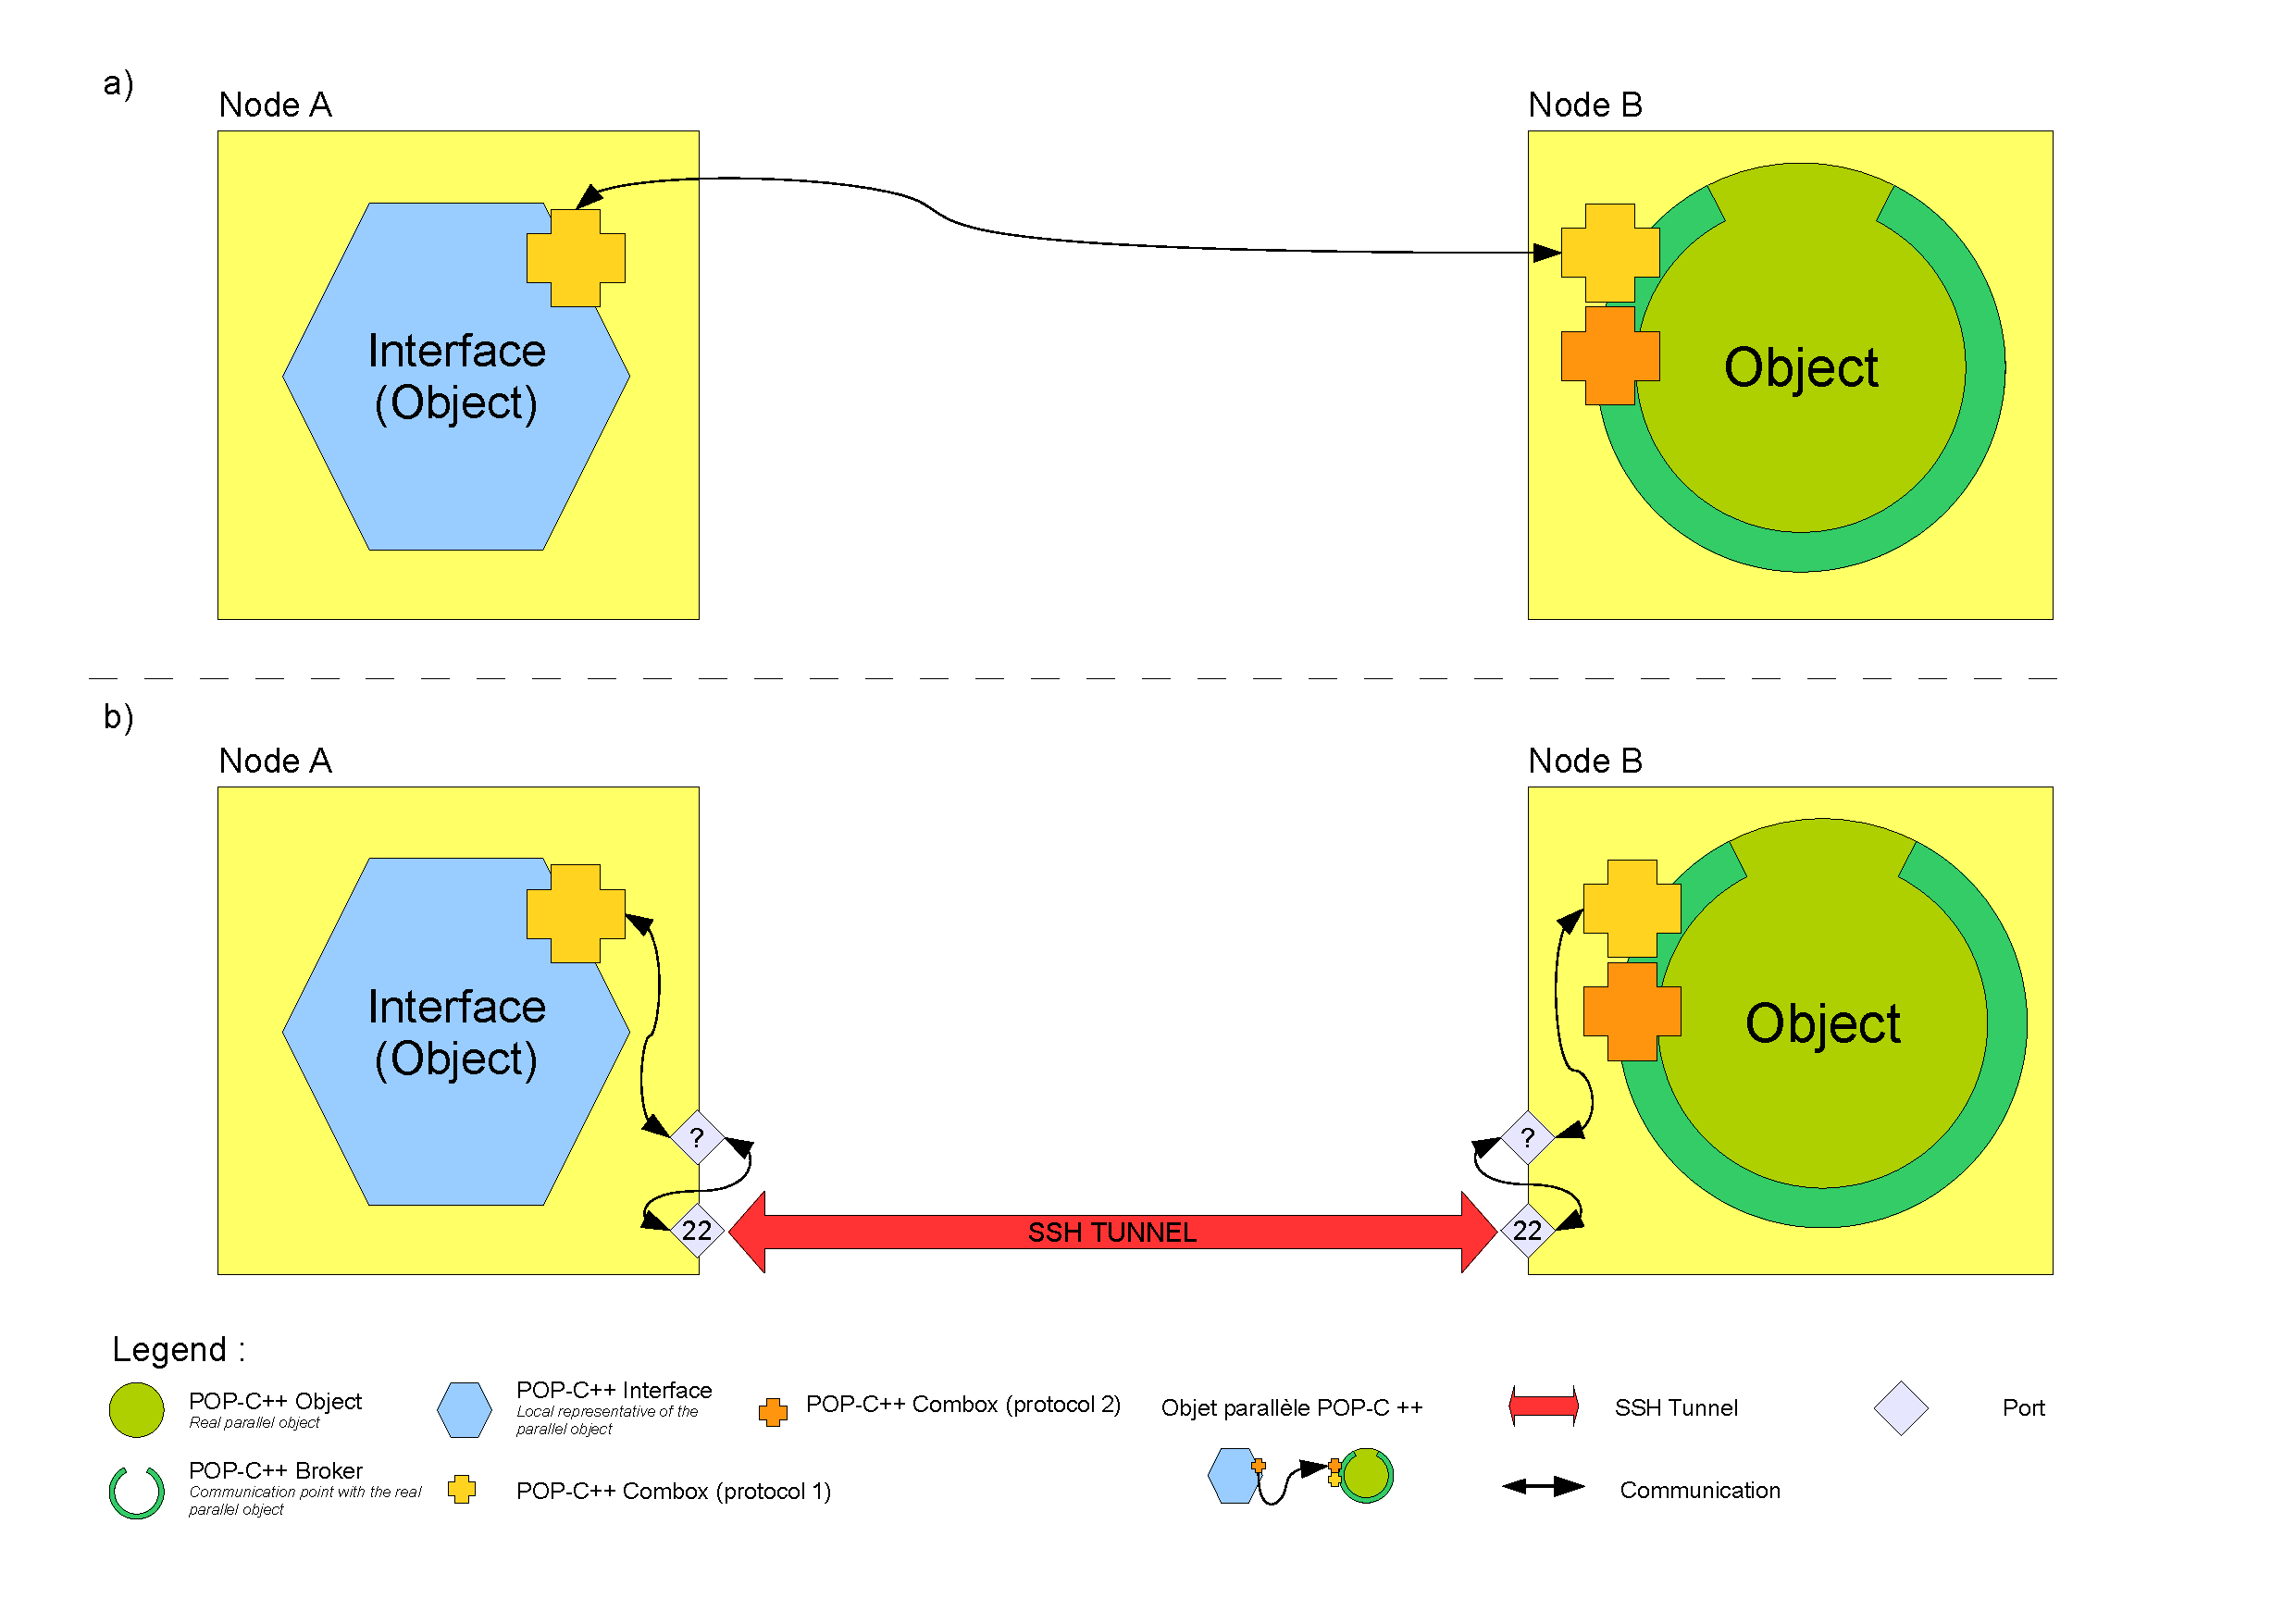
\includegraphics[width=0.9\textwidth]{../std_sec_comm.pdf}
	\label{fig:std_sec_comm}
\end{figure}\vspace{2cm}
\pagebreak

In Figure \ref{fig:std_sec_comm}b, the connection between the interface and the broker is secured by a SSH tunnel. The interface will contact a port on the local machine. This port is redirected through the SSH tunnel to the right remote host address and port.


\subsection{Requirements to use the SSH tunneling}
In order to be able to use the SSH tunneling between an interface and a broker, there are several needs to automatically establish the connection. These needs are listed below : \s
\begin{itemize}
\item The nodes must run a SSH server (e.g. OpenSSH).
\item The port 22 must be opened on the node.
\item If there are any firewalls between nodes, the port 22 must also be opened.
\item The option "StrictHostKeyChecking" must be set to "no". The SSH server will be able to add automatically the new hosts in the file \$HOME/.ssh/known\_hosts.
\item The public key must be exchanged between the two nodes included in a communication.
\end{itemize}\s
The only need that can be done during the installation of POP-C++ is the exchange of the public keys. This exchange process will be explained in Chapter \ref{chap:key_exchange} on page \pageref{chap:key_exchange}.


\subsection{SSH files}
SSH is using public and private keys to authenticate a communication. These keys can be generated with the command \textbf{ssh-keygen}. All the files needed by the SSH process are located in the directory \textbf{\$HOME/.ssh}. This directory contains the following files :  \begin{itemize}
\item \textbf{known\_hosts} : This file stores all the public keys of known nodes.
\item \textbf{id\_rsa} : This file contains the private key. This file must never be exchanged with another node. 
\item \textbf{id\_rsa.pub} : This file contains the public key.
\item \textbf{authorized\_keys} : This file contains the public keys of the nodes that can authenticate automatically to this node.
\end{itemize} 


\subsection{Confidence link in POP-C++}
In order to establish a secure connection between two nodes running POP-C++, they need to have a confidence link between them. This link confirms that one node allows another node to contact him with a secure connection. \\
In our case, the confidence link is established by the exchange of the public SSH keys. Currently, this exchange must be done by hand during the installation of the infrastructure. Only the linked nodes must exchange their key.



\pagebreak
\section{Situation in POP-C++}



In the current version of POP-C++, several connections are made between interfaces and brokers. These connections are the following : 
\begin{enumerate}
\item JobMgr to JobMgr : a JobMgr contacts other JobMgr to register itself to them.
\item PSN to PSN : The POPCSearchNode (PSN) contacts other PSN to discover resources.
\item Object Interface to Object Broker : The interface of a parallel object contacts its broker to perform method calls.
\item Parallel object to Application Services : The parallel object might contact the Application Services to use the Remote Log Service, the Object Monitor Services ...
\end{enumerate}

Figure \ref{fig:crt_sit} shows the communications established during the execution of a POP-C++ application with two parallel objects. This application is using five remote connections during its execution. The local communications will not be secured as they do not send data over the network.

\begin{figure}[ht]
	\caption{Current situation in POP-C++}
  	\centering
	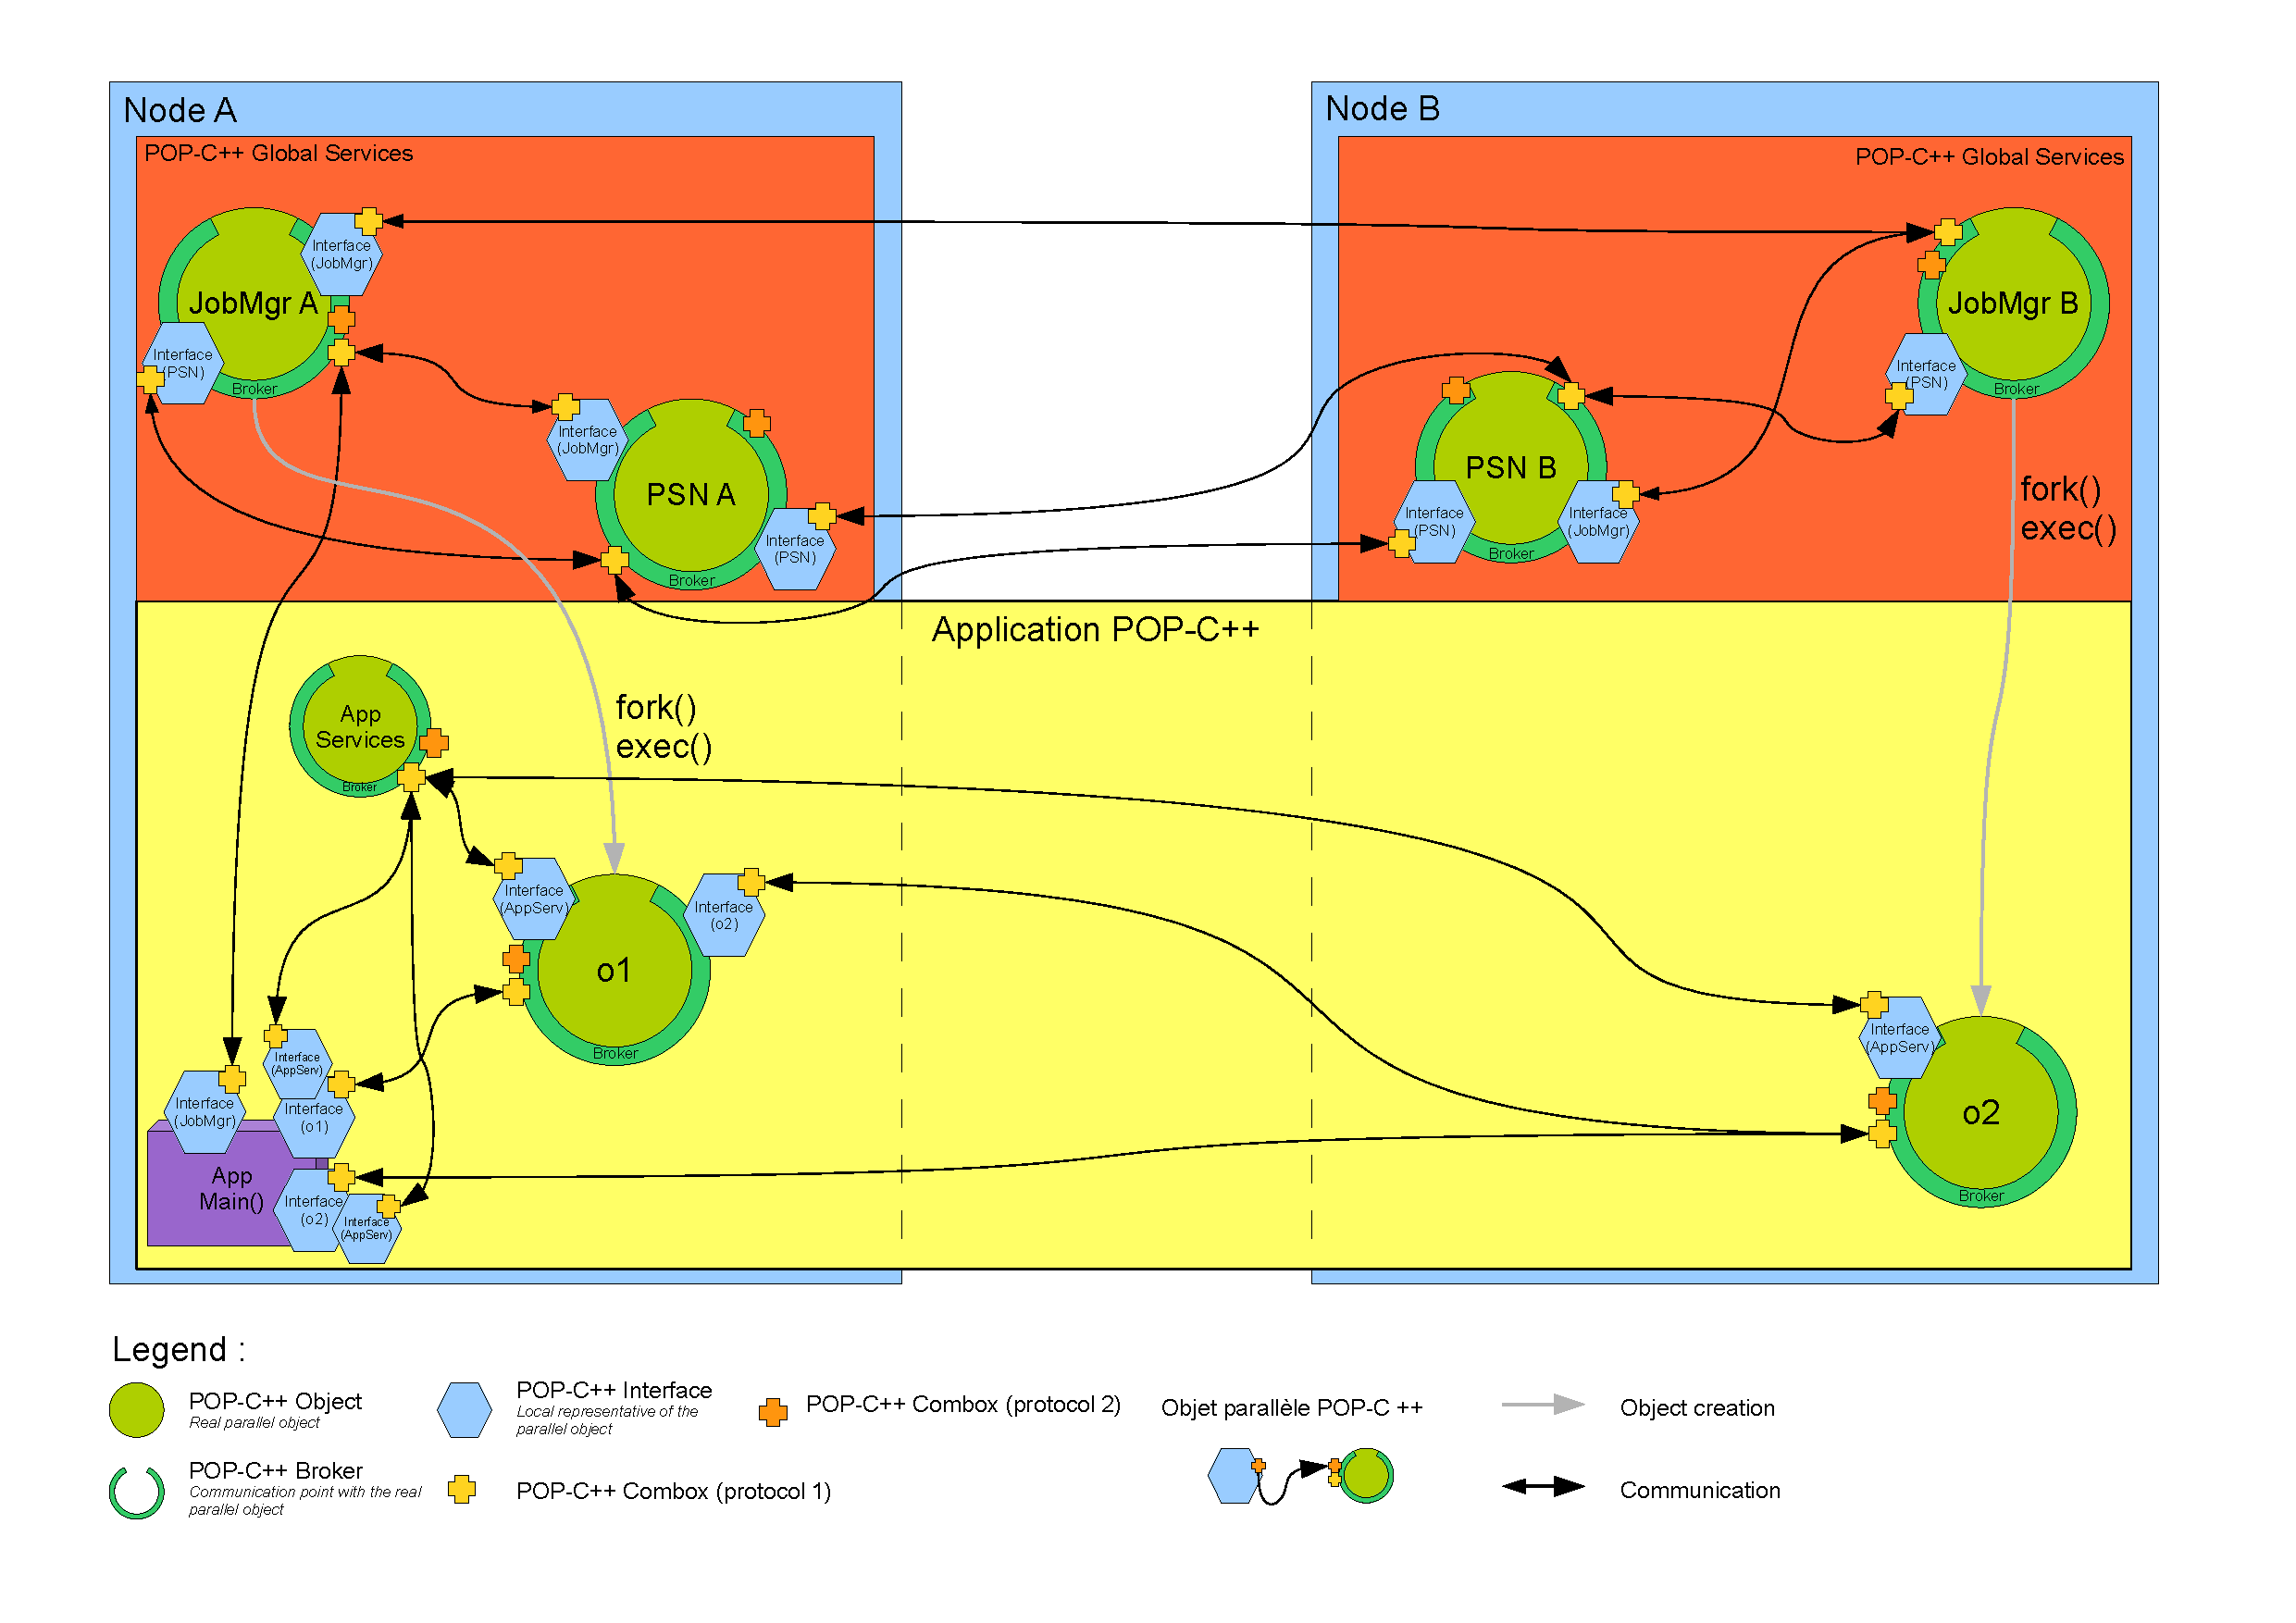
\includegraphics[width=1.0\textwidth]{../popc_crt_situation.pdf}
	\label{fig:crt_sit}
\end{figure}

\textit{NOTE:} The connection is always initiated from an interface to a broker.
\pagebreak



The new implementation of POP-C++ using SSH Tunnelling must create a SSH Tunnel between each remote connection. As shown in Figure\ref{fig:final_sit}, at least four SSH Tunnels are needed to secure the same application. In fact, each parallel objects are listening to different ports. Due to this fact, different SSH tunnels are needed. The interface will connect itself to a local address on a random defined port and the SSH tunnel will automatically redirect this connection to the right remote address and port. All the data sent over the network will be encrypted by the SSH protocol.
\begin{figure}[ht]
	\caption{Final situation in POP-C++}
  	\centering
	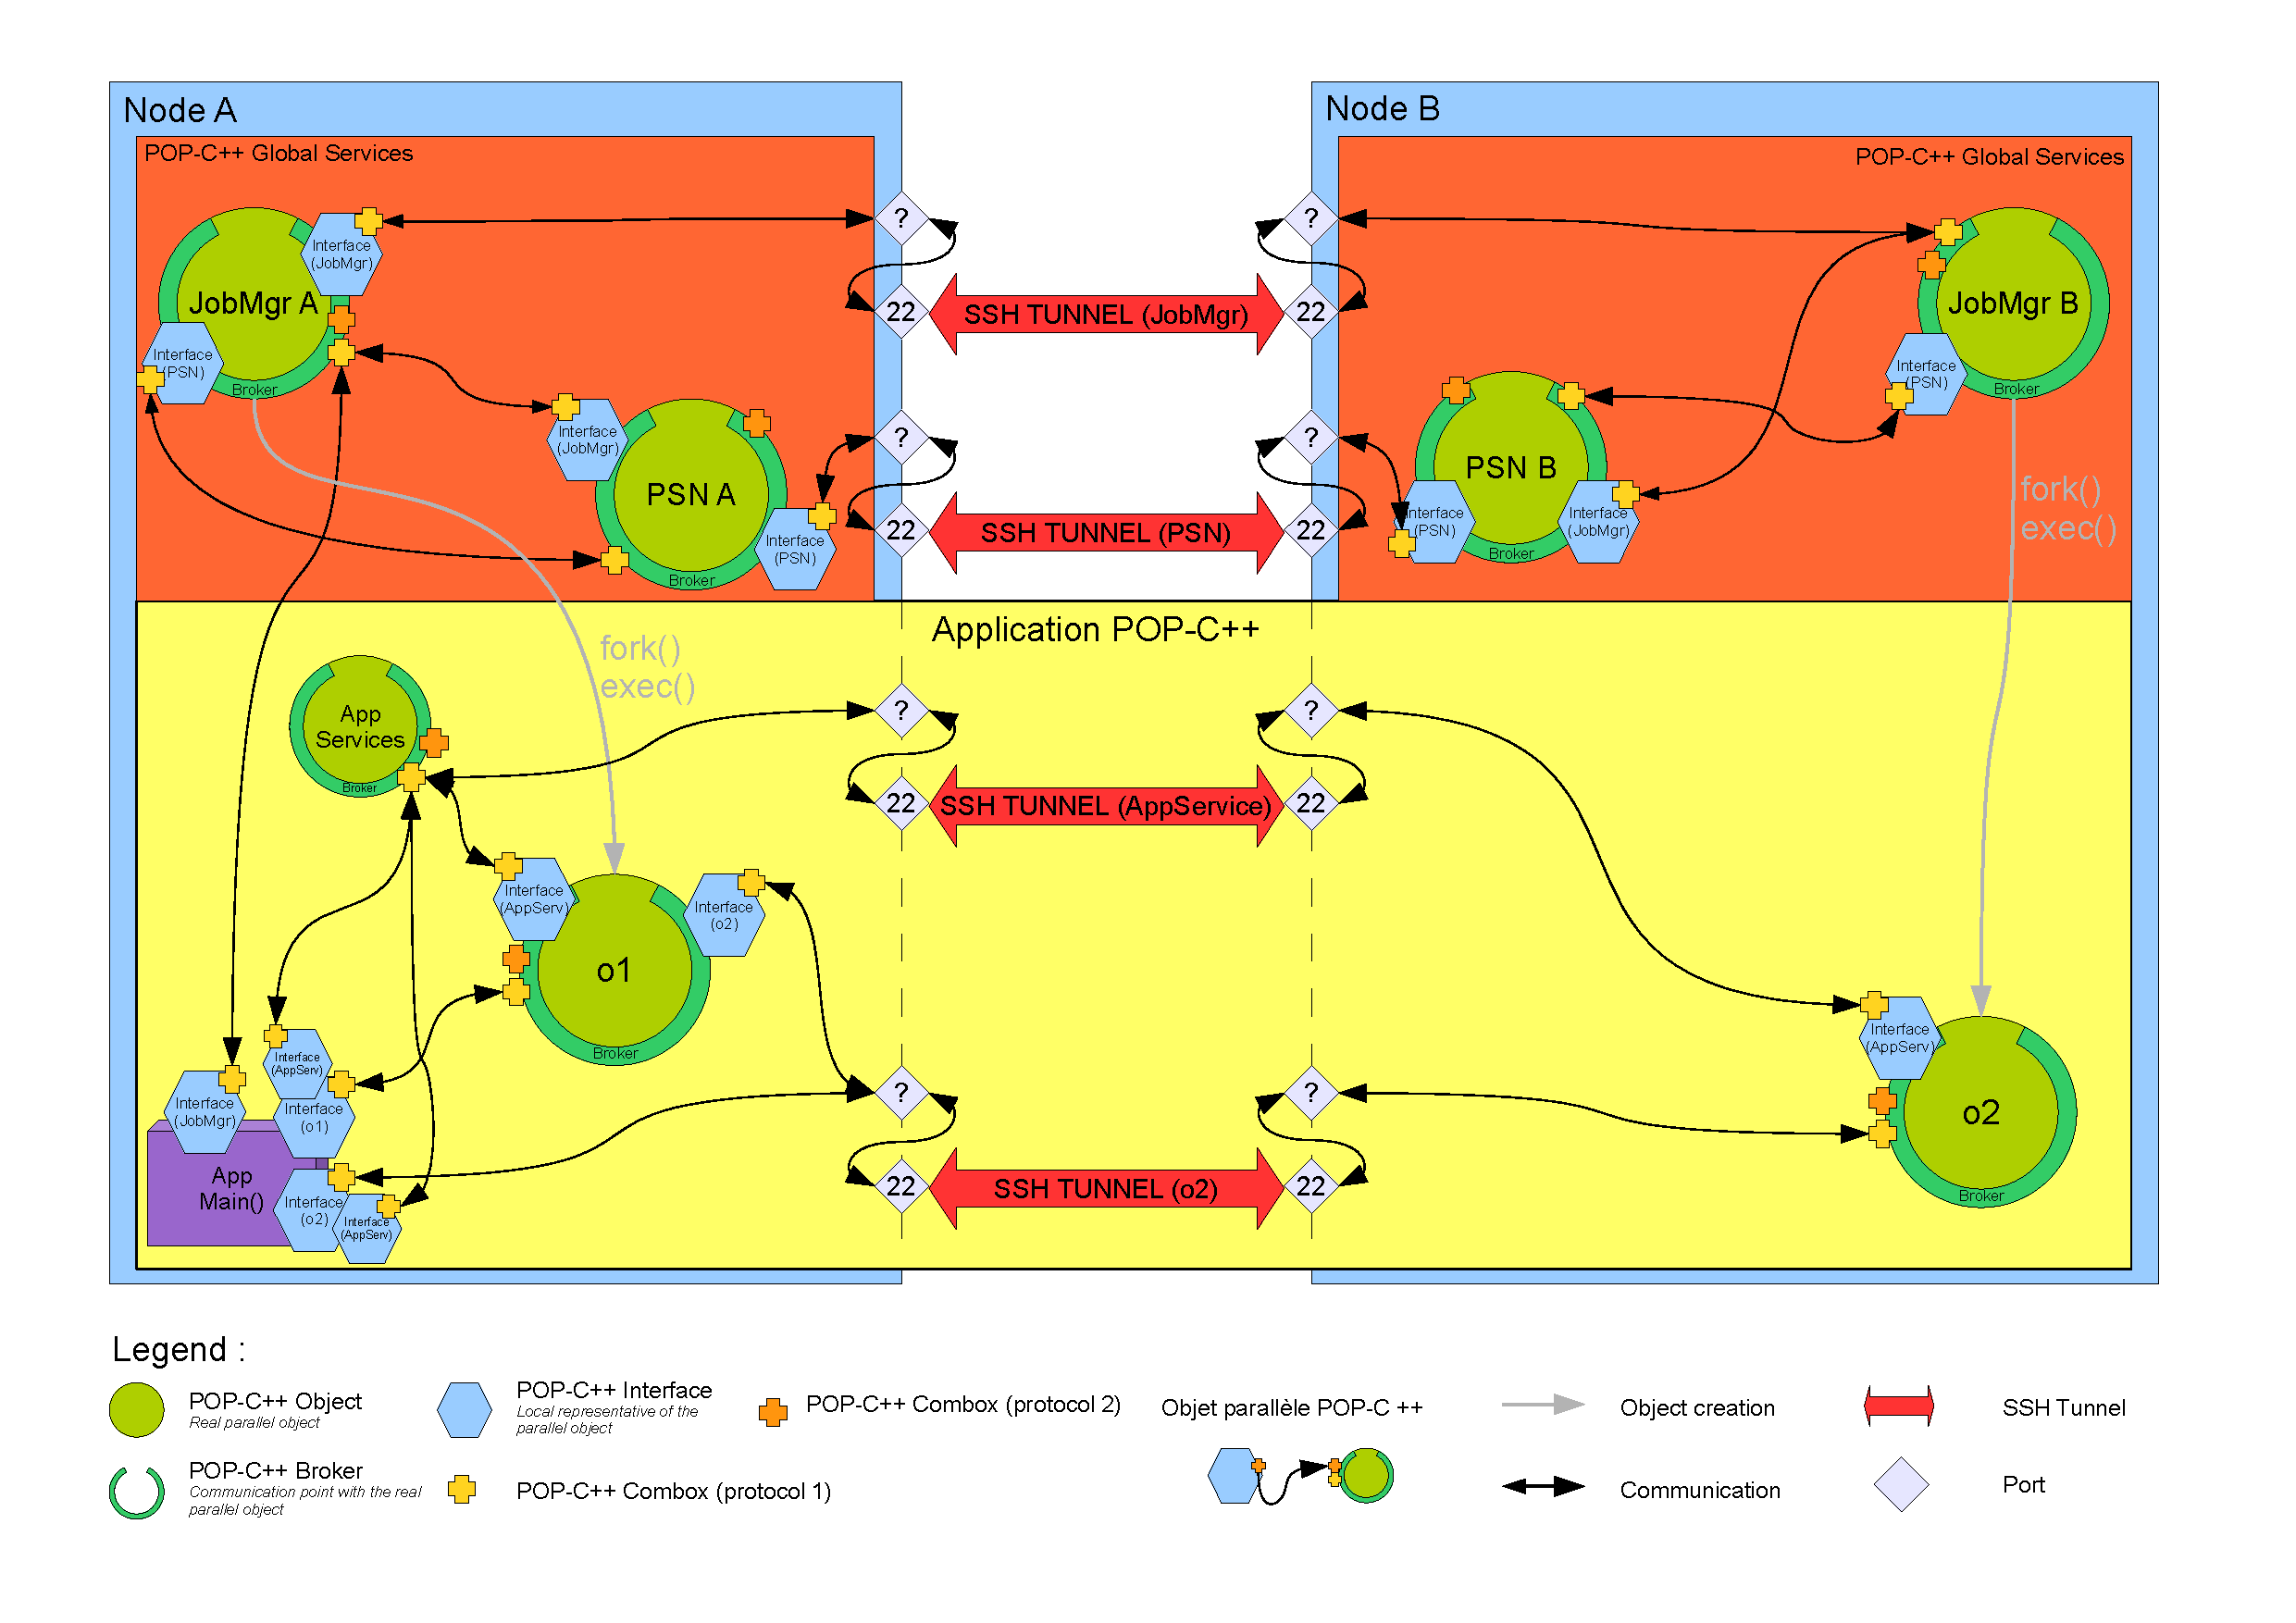
\includegraphics[width=1.0\textwidth]{../popc_final_situation.pdf}
	\label{fig:final_sit}
\end{figure}\vspace{2cm}
\pagebreak
\section{Key exchange process}
\label{chap:key_exchange}


To let all the objects communicate with each other, some public keys must be exchanged during the execution of the POP-C++ application. 
\subsection{Theoretical assumptions}
To be able to implement a version of POP-C++ secured by SSH tunnelling, there are some theoretical assumptions that must be followed.
\begin{enumerate}
\item The main node (the node on which the main program is running) must know all the public keys of every node running a parallel object of the application. This will allow the parallel object to establish a communication with the Application Services running on the main node.
\item The node running a parallel object must know all the public keys of every node which has a reference to this object. This will allow the interface of this parallel object to contact its broker.
\item The node receiving a reference of a parallel object must have the public key of the node who runs this parallel object.
\end{enumerate}




\subsection{Practical point of view}
In a practical point of view, the POP-C++ middle-ware disposes already of some mechanisms that can help the implementation of this security level.\s

\textbf{The access point}\\
The reference of a parallel object is its access point. This access point must hold additional information on the security of the node on which his parallel object is running. The access point must know whether the node must be contacted in a "secure" or "non-secure" way. \\
The access point must also hold the public key of the node on which his parallel object is running.\s

\textbf{The main program}\\
The node A running the main program must know the public key of the node B running a parallel object of this program. This public key must be given in the response of the resource discovery but it should be used only if the parallel object is created on node B.


\pagebreak
\subsection{Scenario}
In this section, there are two scenarios fully explained to understand the whole process of the key exchange in POP-C++. 

\subsubsection{Scenario 1}
In the first scenario illustrated Figure\ref{fig:kex_object_creation} and Figure\ref{fig:kex_ref_passing}, there are 7 nodes running POP-C++. The node "M" is the main node running the "main" of the POP-C++ application.\\
The object creation goes as follow : \s

\begin{enumerate}
\item The main node "M" creates the parallel object "o1" on the node "A" and the parallel object "o4" on the node "D".
\item The object "o1" in Node "A" creates the parallel object "o2" on the Node "B".
\item The object "o2" in Node "B" creates the parallel object "o3" on the Node "C".
\item The object "o4" in Node "D" creates the parallel object "o5" on the Node "E".
\item The object "o5" in Node "E" creates the parallel object "o6" on the node "F".
\end{enumerate}\s

\emph{NOTE:} When an object creates another object, the JobMgr on the node running the object will be contacted.\s

During its creation, a parallel object must give its public key to the main node. After the whole object creation process, the main node will know the public keys of all nodes. \s

When a parallel object is created from another parallel object, the node who creates the object must know the public key of the node who runs the parallel object. This will allow the interface to contact the broker with a secure connection.
\begin{figure}[ht]
	\caption{Scenario 1 : Key exchange during objects creation}
  	\centering
	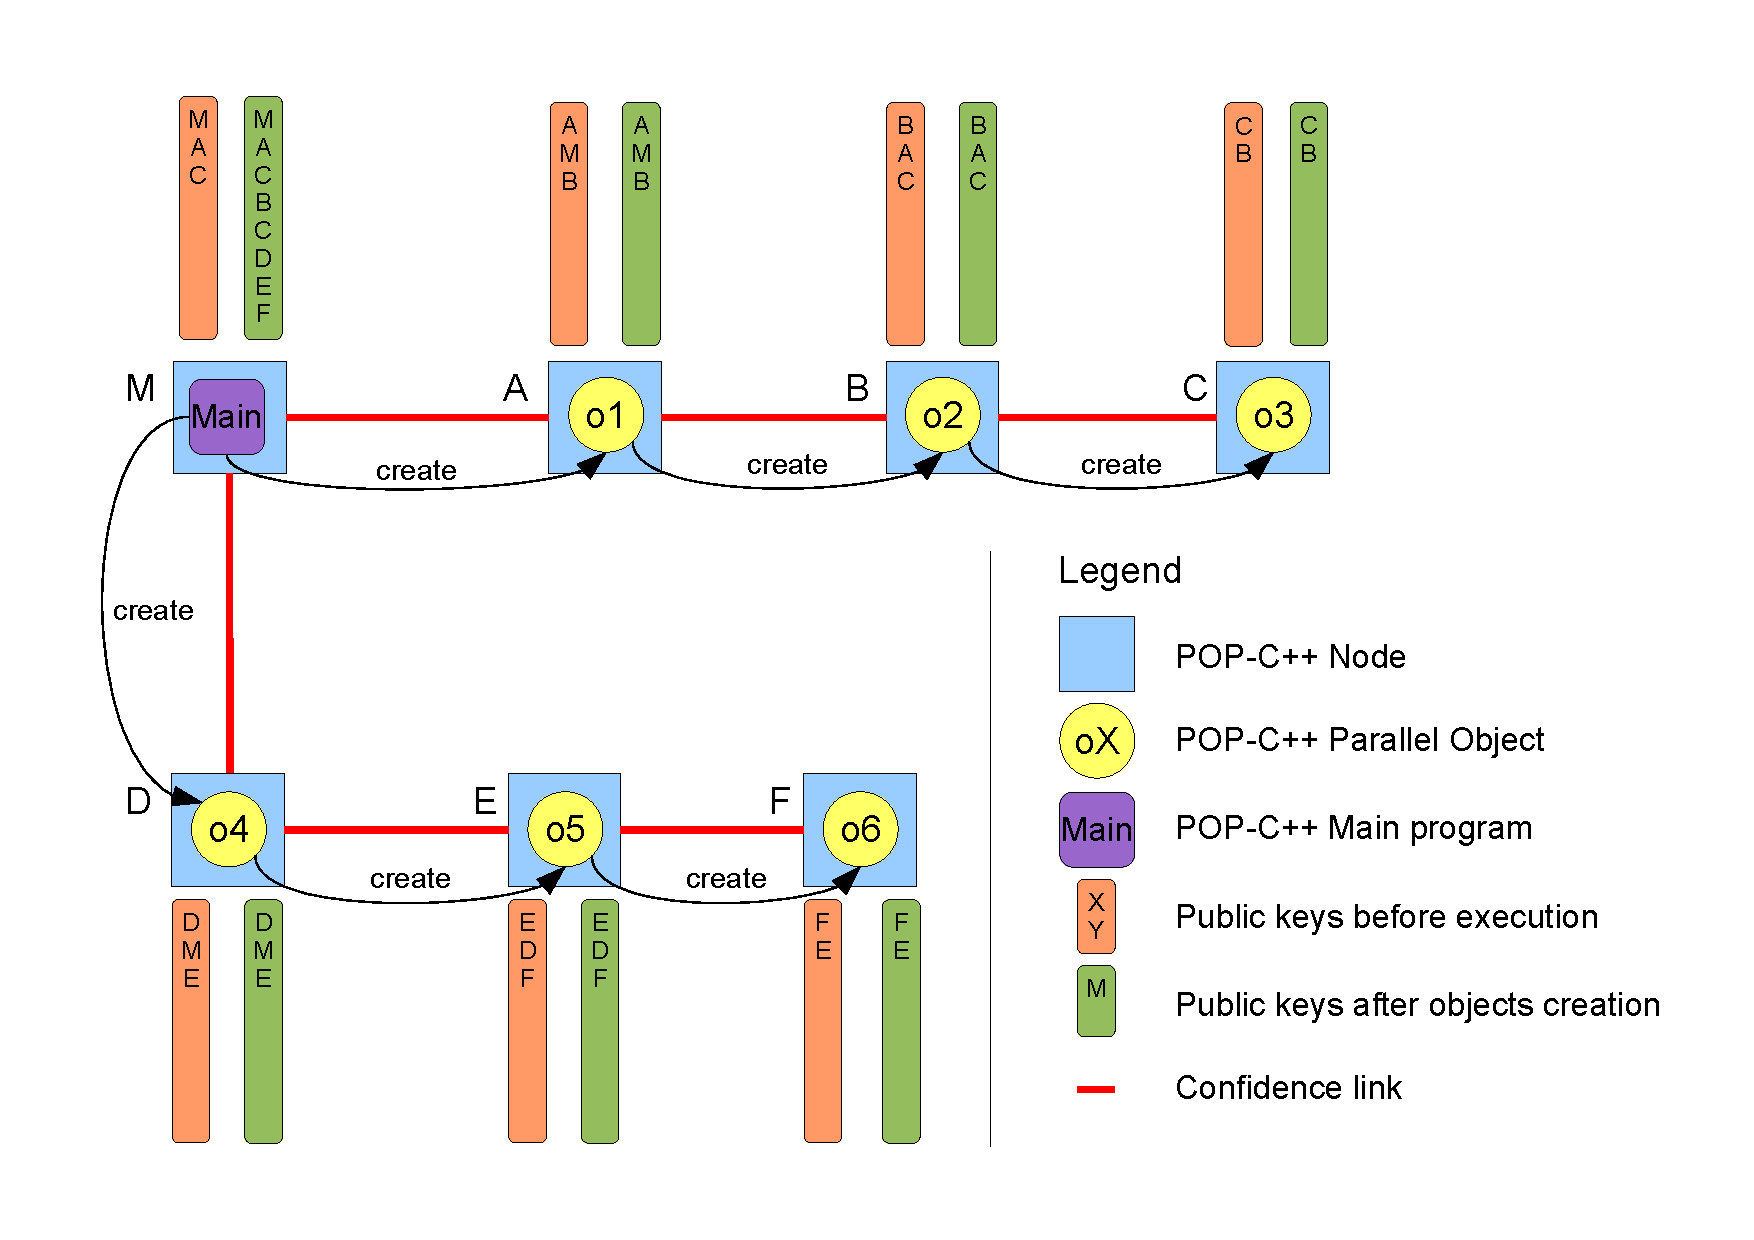
\includegraphics[width=0.7\textwidth]{../object_creation.pdf}
	\label{fig:kex_object_creation}
\end{figure}



\pagebreak


Figure \ref{fig:kex_ref_passing} shows the passing of parallel object reference between parallel objects. This procedure is explained below : 
\begin{enumerate}
\item The node "A" passes the reference of "o2" to the main node. The node running "o2" adds the public key of "M". The node "M" adds the public key of the node running "o2".
\item The node "M" passes the reference of "o2" to the node "D". The node running "o2" adds the public key of "D". The node "D" adds the public key of the node running "o2".
\item The node "D" passes the reference of "o2" to the node "E". The node running "o2" adds the public key of "E". The node "E" adds the public key of the node running "o2".
\item The node "E" passes the reference of "o6" to the node "B". The node running "o6" adds the public key of "B". The node "B" adds the public key of the node running "o6".
\end{enumerate}
\begin{figure}[ht]
	\caption{Scenario 1 : Key exchange during reference passing}
  	\centering
	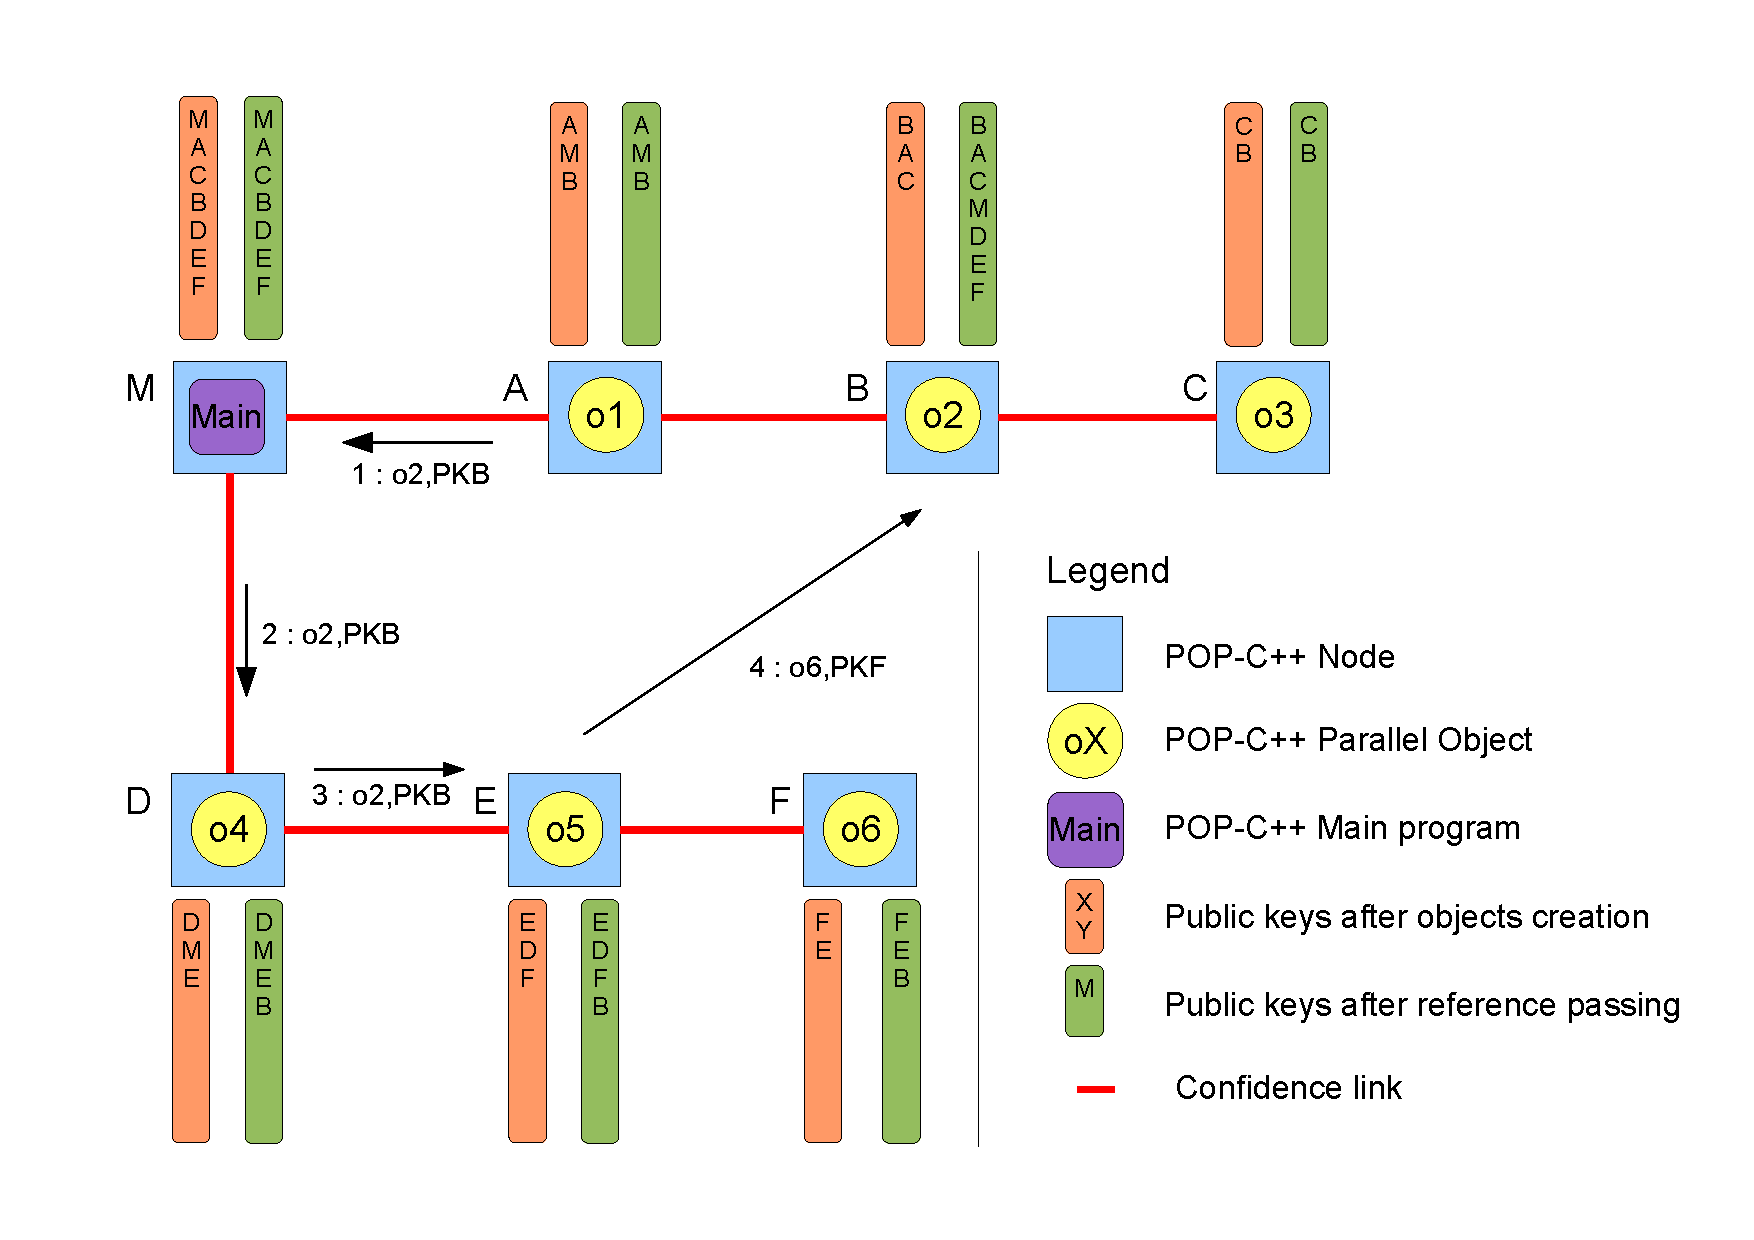
\includegraphics[width=0.8\textwidth]{../ref_passing.pdf}
	\label{fig:kex_ref_passing}
\end{figure}

\pagebreak
\subsubsection{Scenario 2}
In the second scenario, there are 8 nodes running POP-C++. The node running the "main" of the POP-C++ application is the node "C". The objects creation goes as follows : 
\begin{itemize}
\item The node "C" will create the objects "o1", "o5" and "o6". 
\item The node running "o1" will create the objects "o2" and "o4". 
\item The node running "o2" will create the object "o3".
\item The node running "o6" will create the object "o7".
\end{itemize}
Like in the first scenario, the main node will know all the public key. All the parallel objects will be able to communicate with the "Application Services" located on the main node.\\
The node who creates a parallel object gives his public key to the node running this parallel object. This allows the interface to communicate to the broker trough a secure link. 

\begin{figure}[ht]
	\caption{Scenario 2 : Key exchange during objects creation}
  	\centering
	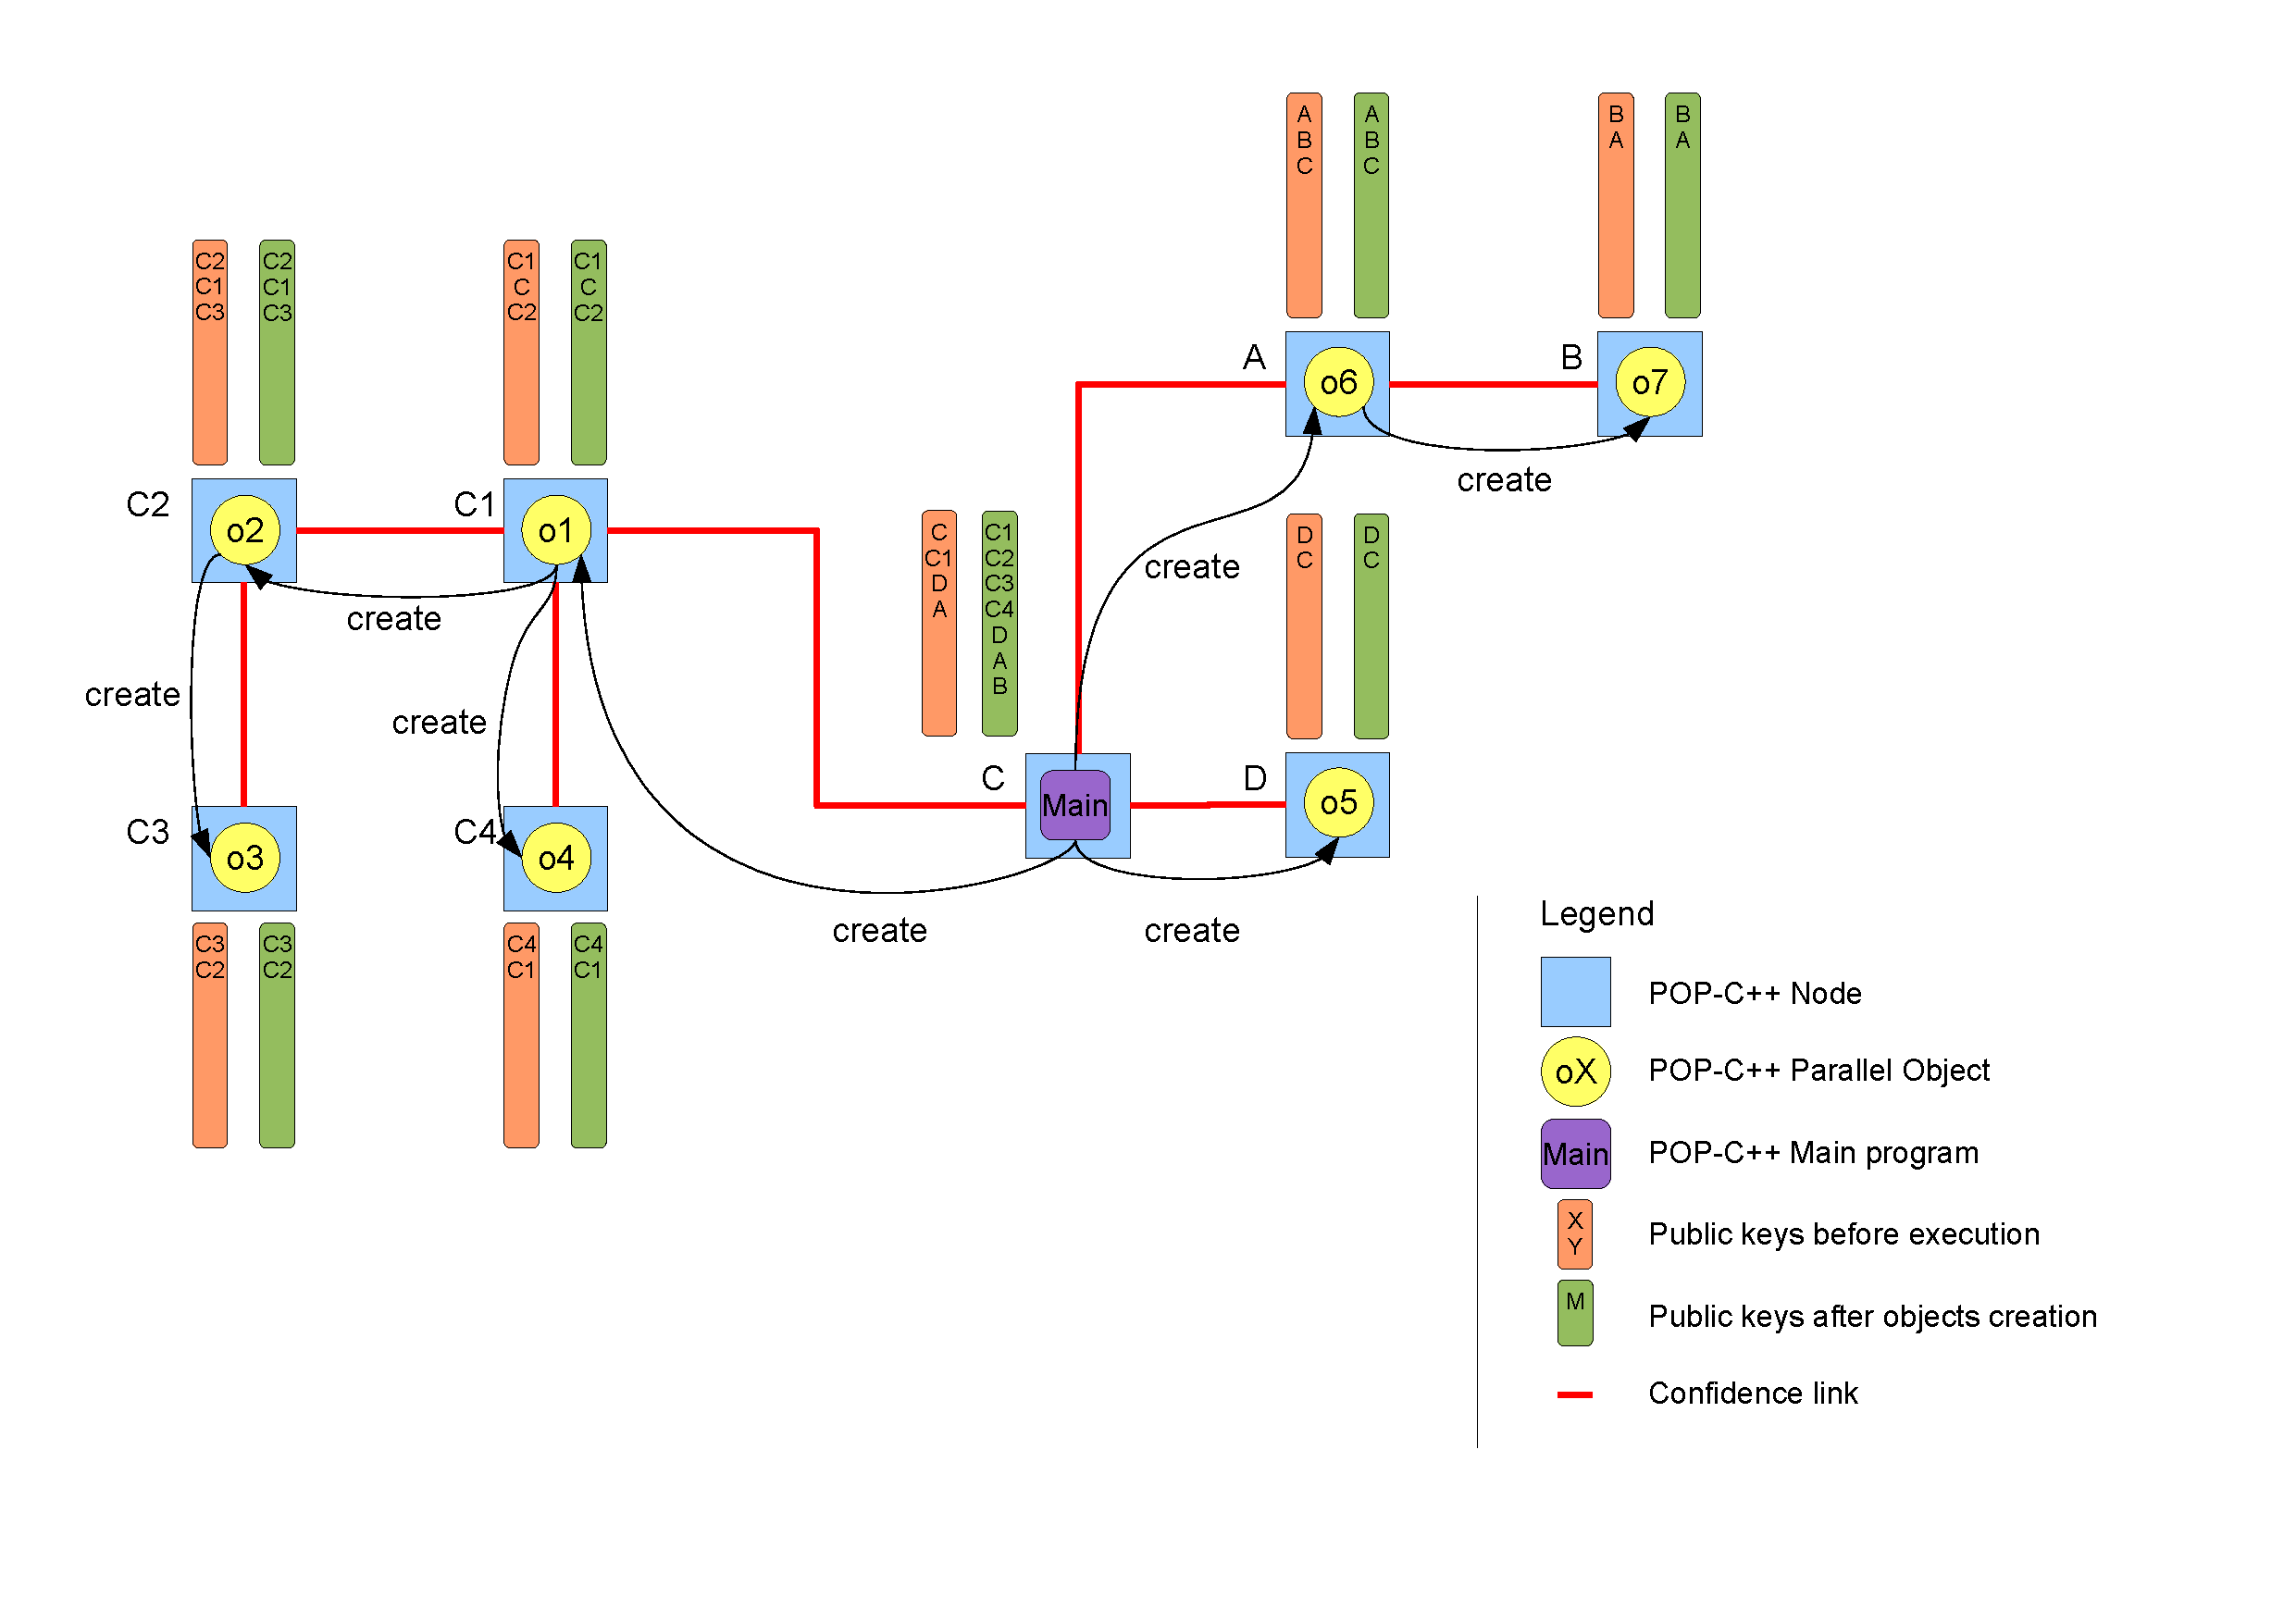
\includegraphics[width=1.0\textwidth]{../sc2-1.pdf}
	\label{fig:kex_object_creation_sc2}
\end{figure}
Once the parallel object creation is done, the program can pass references of parallel object to another parallel object.

\pagebreak

\begin{figure}[ht]
	\caption{Scenario 2 : Key exchange during reference passing}
  	\centering
	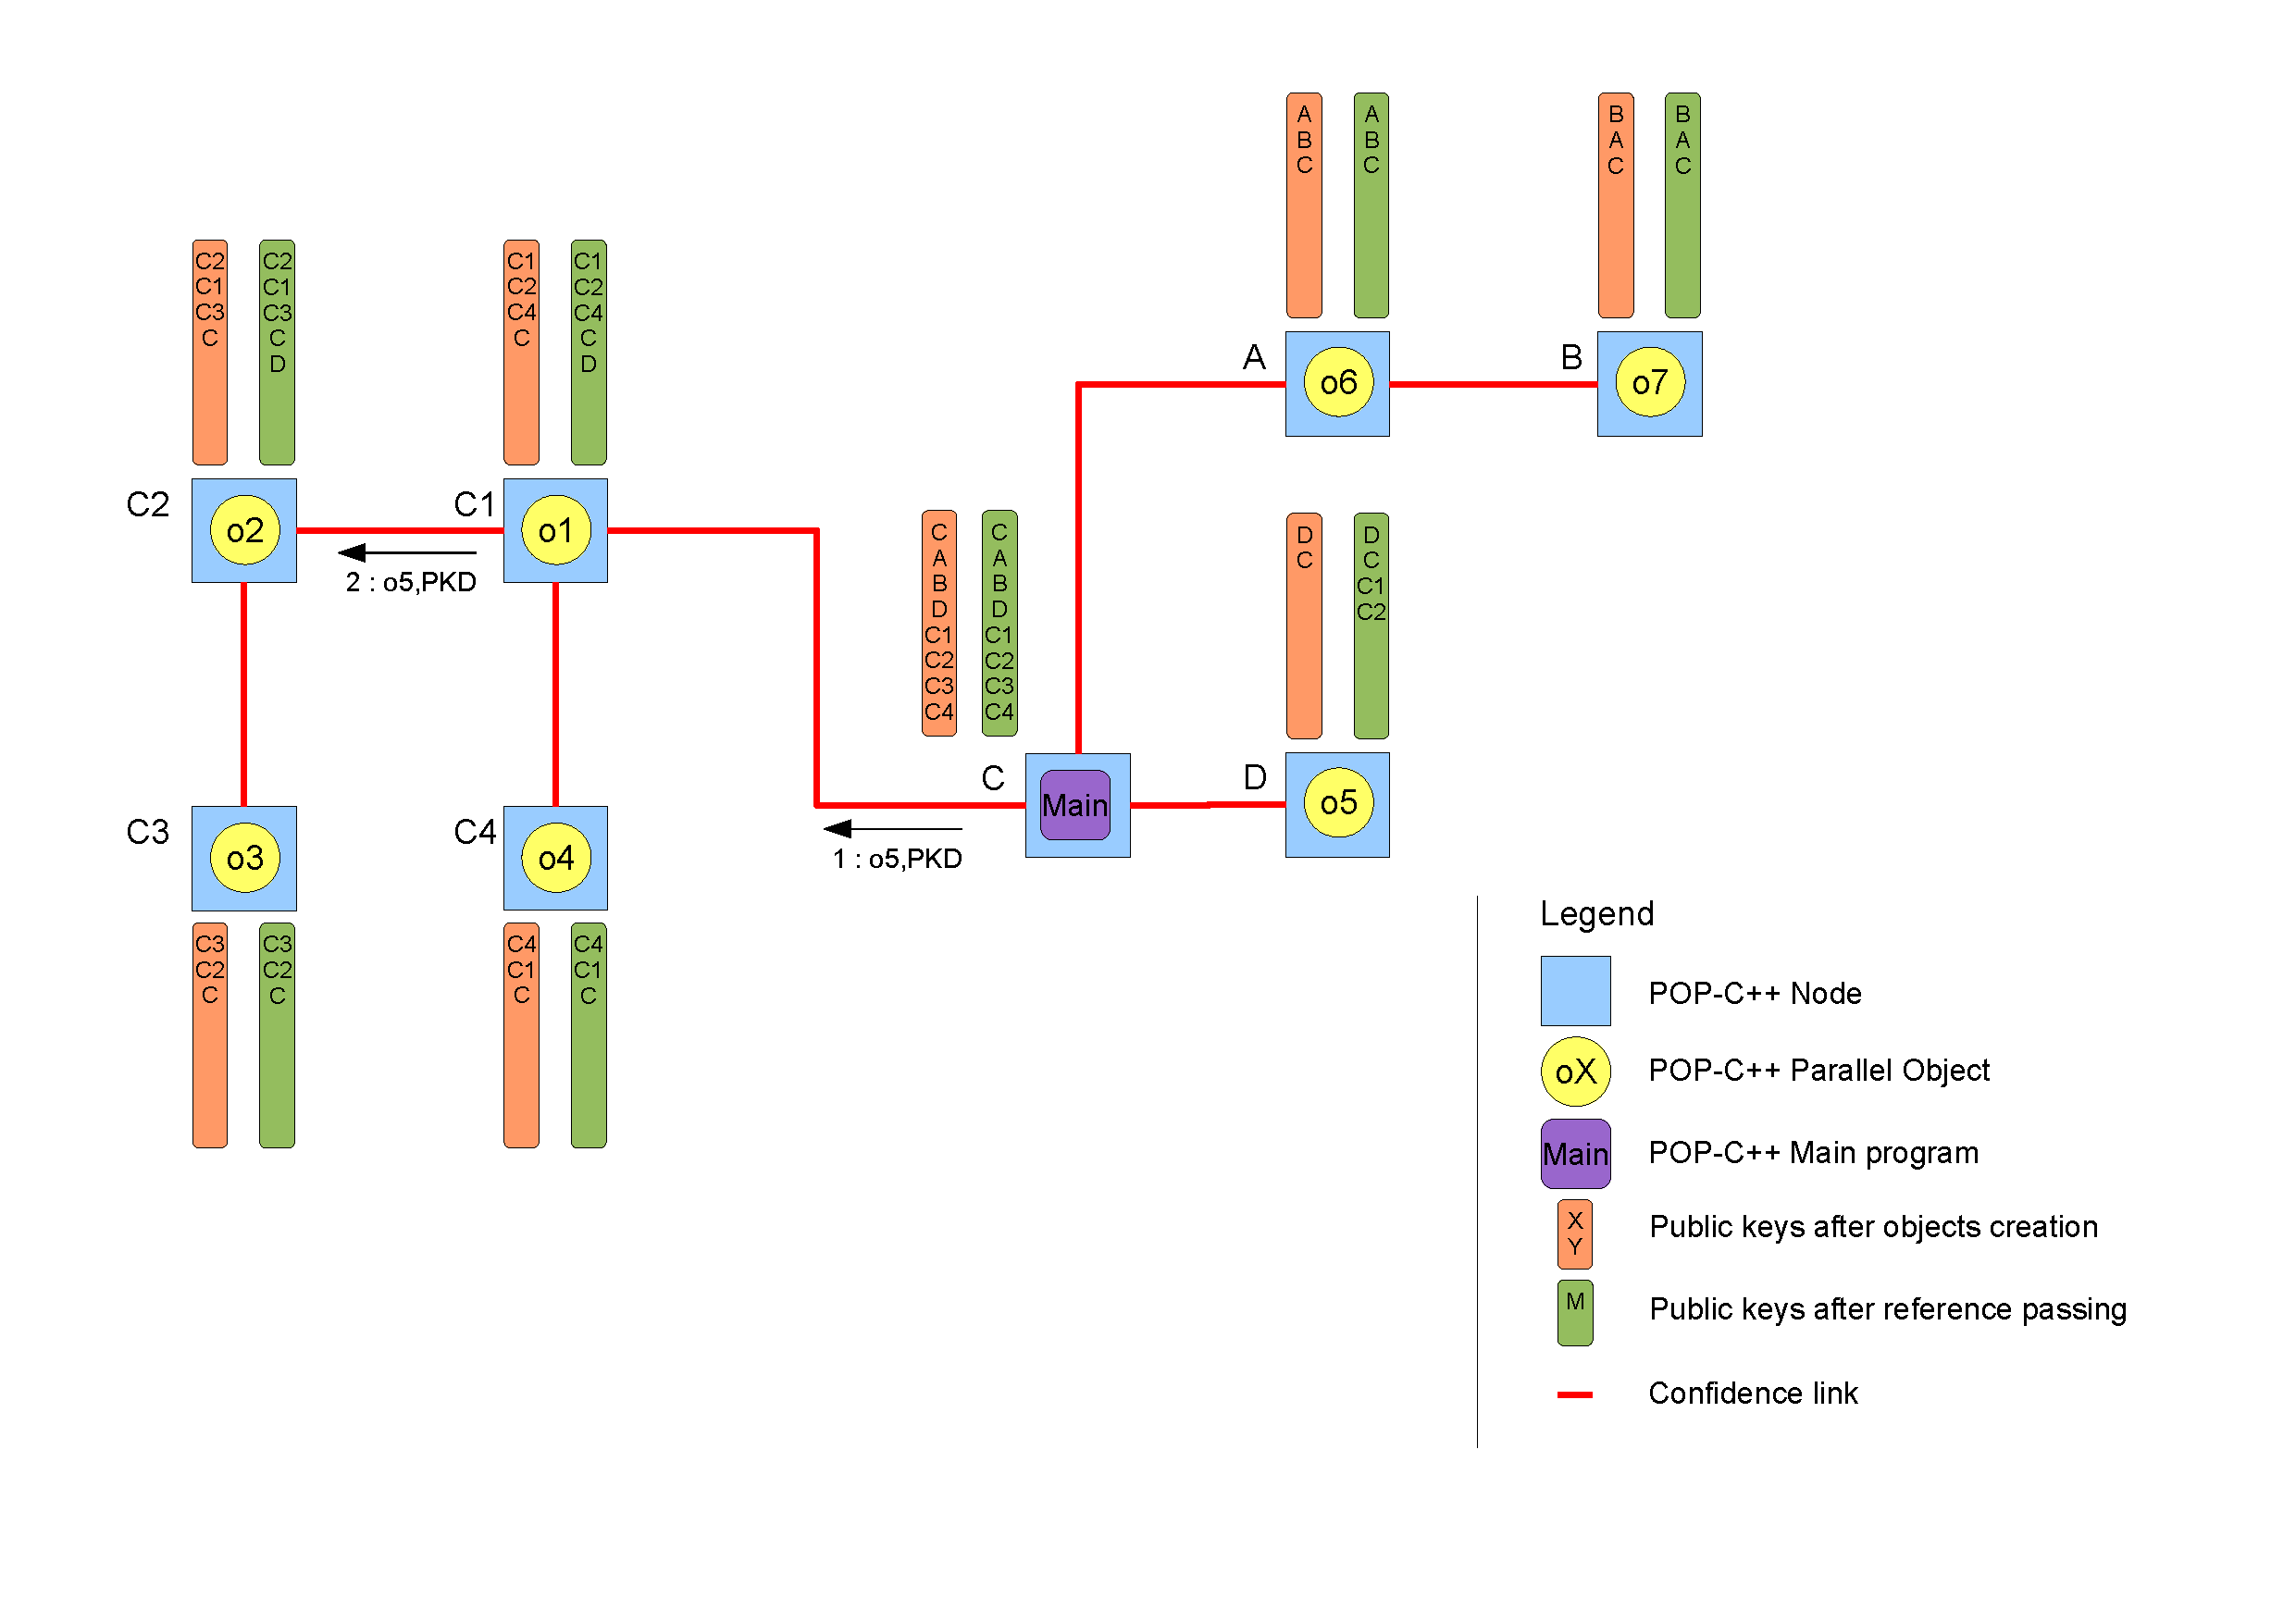
\includegraphics[width=1.0\textwidth]{../sc2-2.pdf}
	\label{fig:kex_ref_passing_sc2}
\end{figure}

In this scenario, the reference of the object "o5" is passed to the node "C1" and after to the node "C2". This reference passing goes like this : \s

\begin{enumerate}
\item The node "C" passes the reference of "o5" to the node "C1". The node running "o5" adds the public key of "C1". The node "C1" adds the public key of the node running "o5".
\item The node "C1" passes the reference of "o5" to the node "C2". The node running "o5" adds the public key of "C2". The node "C2" adds the public key of the node running "o5".
\end{enumerate}\s

The node "C2" is now able to communicate with the parallel object "o5" because the node can create a SSH tunnel between him self and the node "D".
\pagebreak
\pagebreak
\section{Implementation in POP-C++}
This chapter is full review of the modifications made to POP-C++ to make a secure version using the SSH tunnelling. \s

\emph{REMARK:} This work is based on POP-C++ 1.3.1 beta J1 version of the POP-C++ middle-ware.\s

\textit{NOTE : } All the code added for this specific version if preceded by the following comment : 

\begin{lstlisting}
/**
 * ViSaG : clementval
 * Comment
 */
\end{lstlisting}


\subsection{POP Application Unique Identifier}
An application needs a unique identifier for several purposes during its execution. The POP App ID is created with the three followings items : 
\begin{itemize}
\item The start-up timestamps.
\item A hash of the challenge string of the current application services.
\item The address of the node running the main program.
\end{itemize}

\textit{NOTE:} The process ID of the main program could also be included in the POP Application Identifier.

The POP Application Unique Identifier could look like this :\\

\begin{center}
\textit{POPAPPID\_1234567\_908767654578\_160.98.21.168}
\end{center}\s

This ID will be used to maintain a mapping between routing informations and an application. It will also be used in the Virtual version of POP-C++. The POP App ID is created by the "Application Scope Services" in the constructor of the "AppCoreService" class.\s

\textbf{File modified:} ./lib/appservice.cc\s

\subsection{POP-C++ Security Manager (PSM)}
To centralize the management of the key exchange, key re-routing and the key writing, a new parallel object is added to the Global Services of POP-C++. This parallel object is the POP-C++ Security Manager (PSM). The class name of this object is "POPCSecurityManager". \s

\textbf{New files :} ./lib/popc\_security\_manager.ph, ./lib/popc\_security\_manager.cc

\pagebreak
\subsubsection{New POP-C++ Global Services vision}
With this new parallel object, the POP-C++ Global Services are now composed of the JobMgr, the POP-C++ Search Node (PSN) and the POP-C++ Security Manager (PSM). Figure \ref{fig:new_gc} shows a schematic view of the POP-C++ Global Services with the intercommunications between them.

\begin{figure}[ht]
	\caption{New Global Services Vision}
  	\centering
	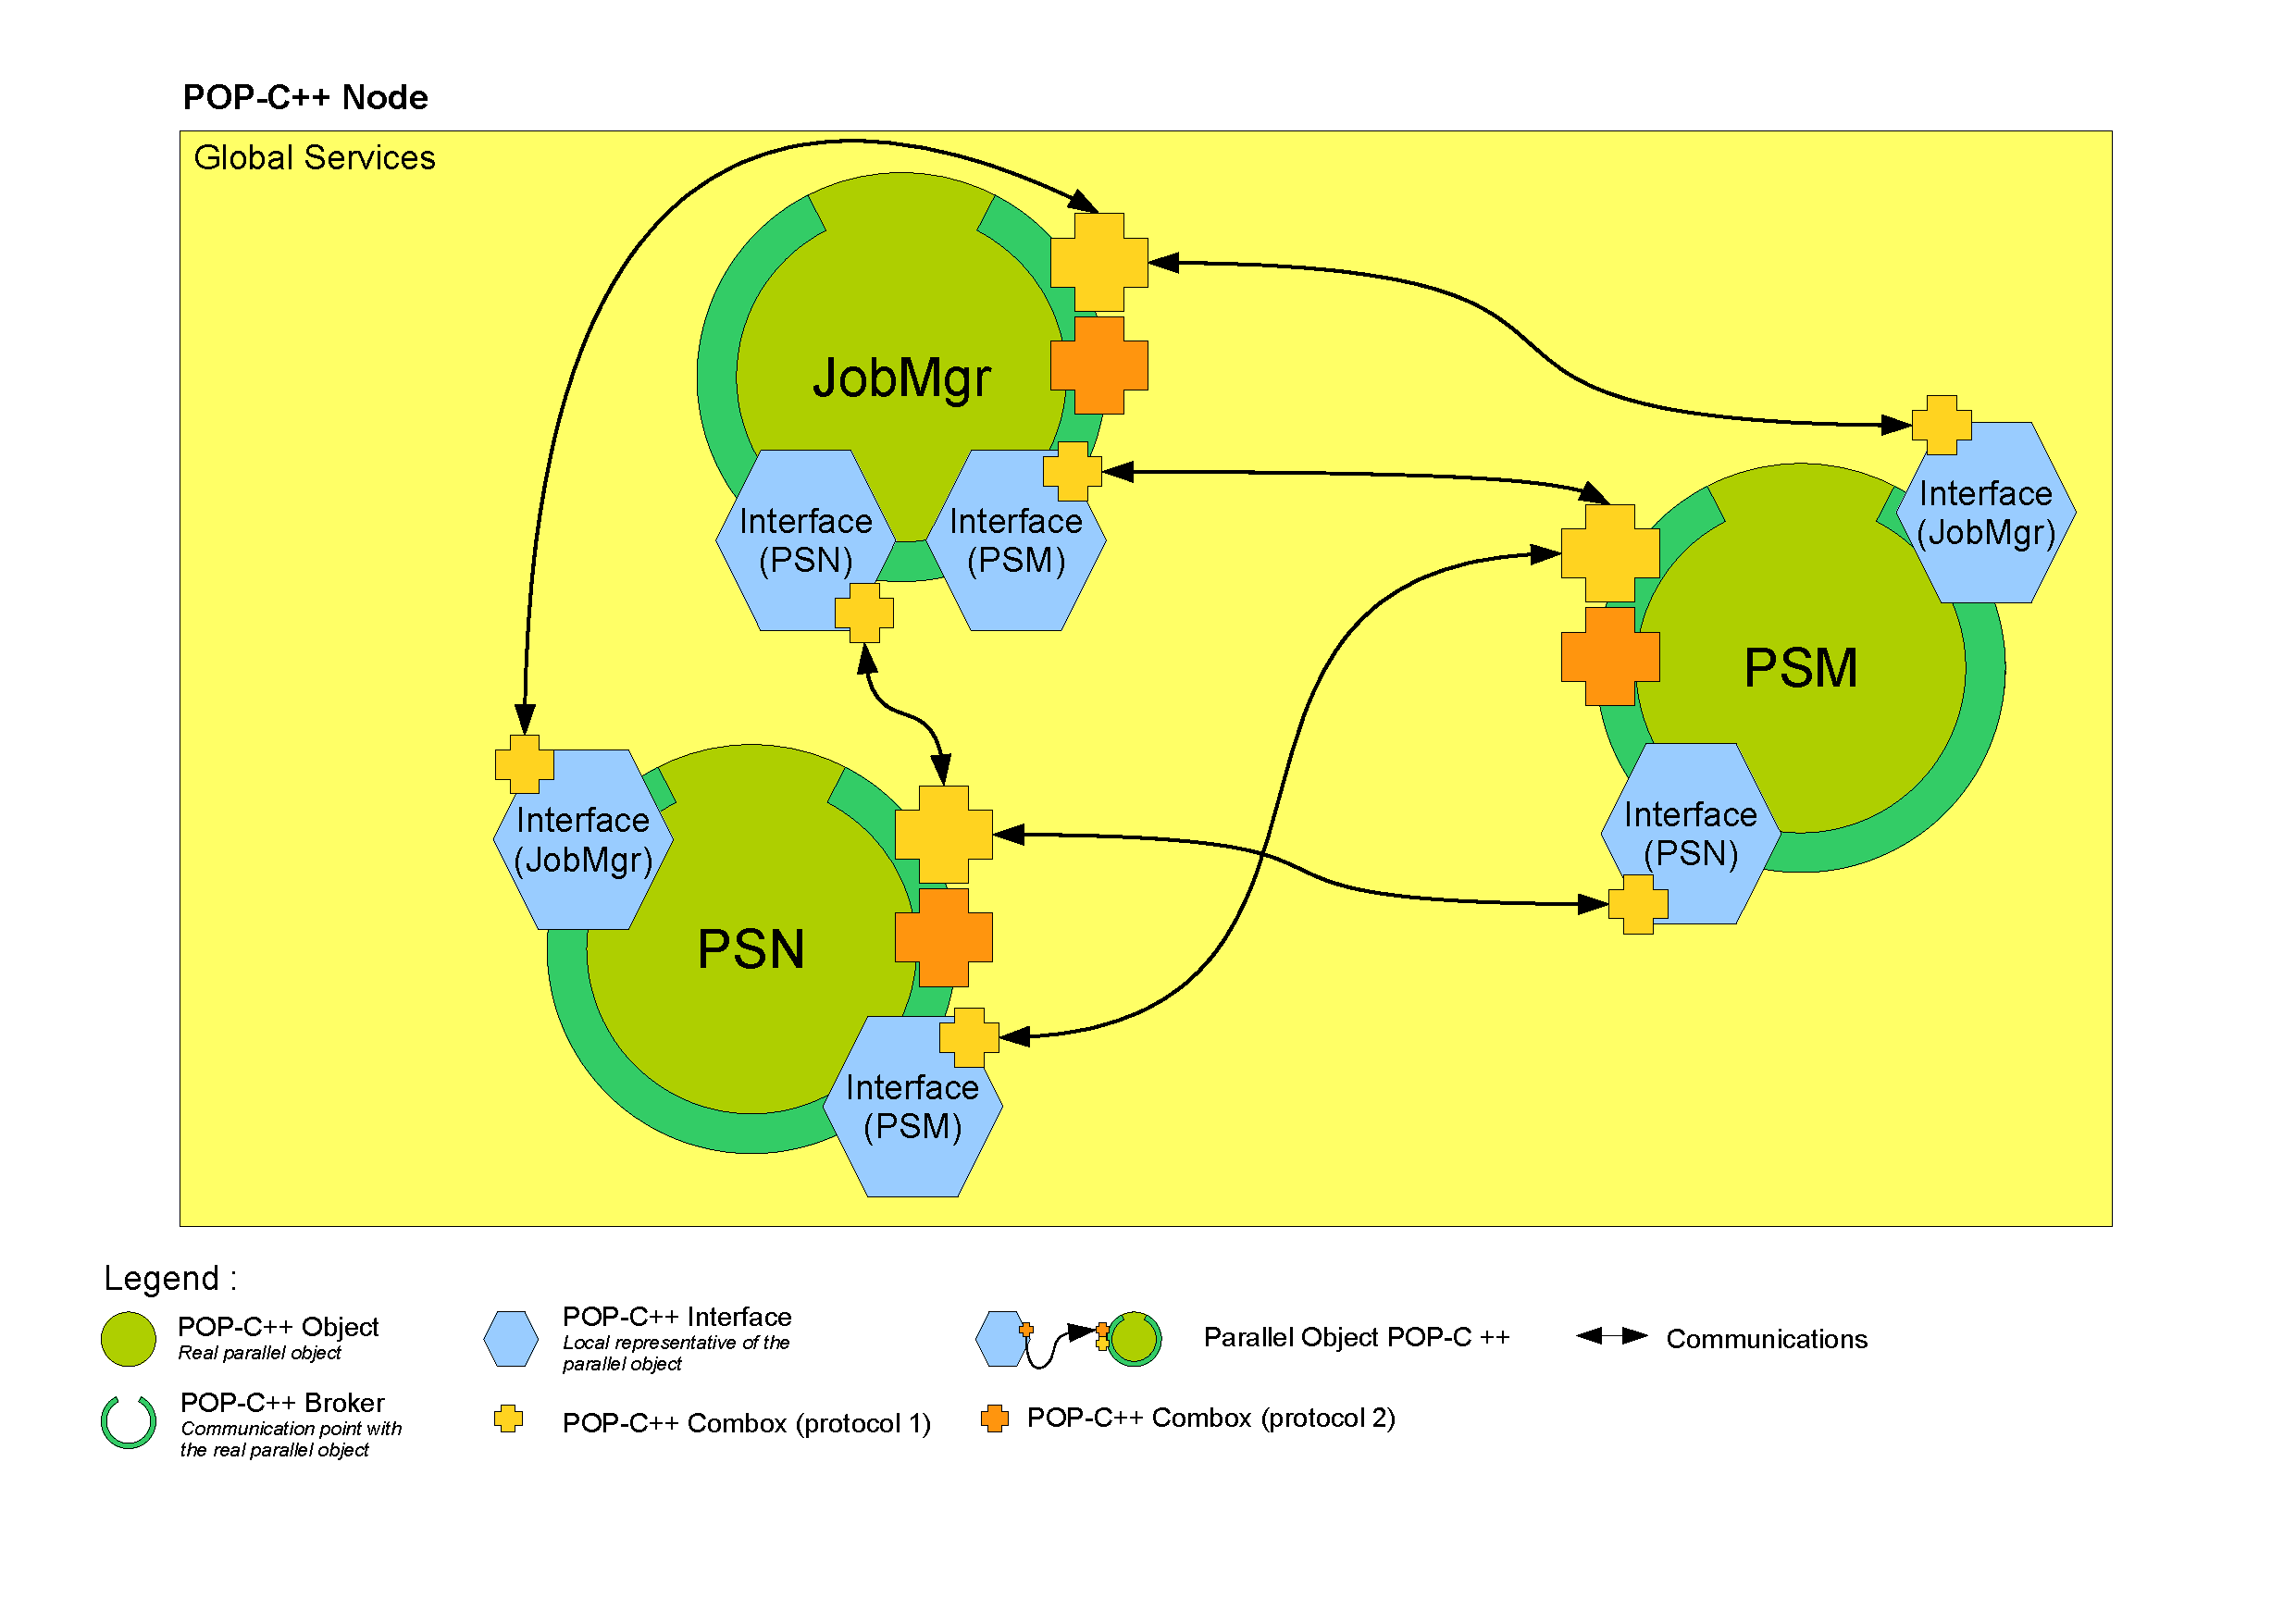
\includegraphics[width=1.0\textwidth]{../global_services.pdf}
	\label{fig:new_gc}
\end{figure}

\pagebreak
\subsubsection{Global Services startup}
The PSM is started with the JobMgr and the PSN. The file POPC\_SOURCES/services/jobmgr\_launcher.cc has been modified to include the new parallel object PSM. The JobMgr constructor has also been modified to be able to pass a reference of the PSM and the PSN to it. Figure \ref{fig:gc_startup} shows the sequence  of the POP-C++ Global Services start-up.

\begin{figure}[ht]
	\caption{Sequence Diagram : Global Services start-up}
  	\centering
	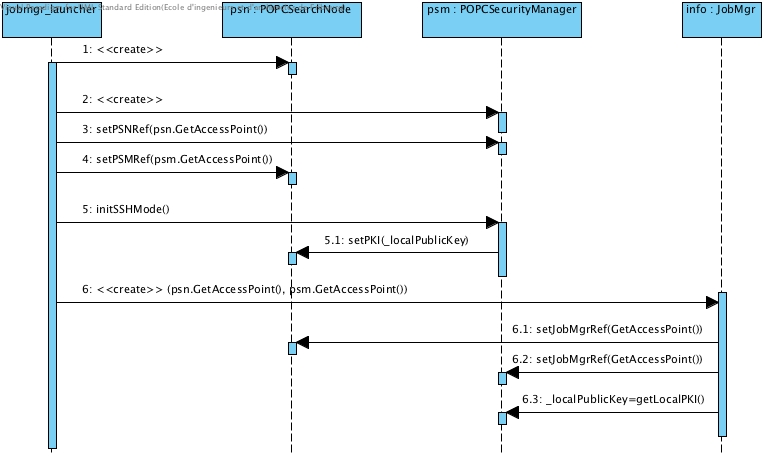
\includegraphics[width=1.0\textwidth]{../gs_startup.jpg}
	\label{fig:gc_startup}
\end{figure}\s

\textbf{Files modified :} ./lib/jobmgr.ph, ./lib/jobmgr.cc, ./lib/popc\_search\_node.ph, ./lib/popc\_search\_node.cc

\subsubsection{POP-C++ Security Manager start-up}
As we can see on Figure \ref{fig:gc_startup}, a method named "initSSHMode()" is called just after the PSM and PSN creation. This method will initialize all the needed variables for the SSH tunnelling. In fact, this method will read the local public key, store it in a variable and then pass it to the local PSN.\s

\textit{REMARK} : In the future, this method will also read the "authorized\_keys" file and keep all the keys in a data structure.

\subsubsection{Mapping}
In the PSM, two different mappings are saved during applications execution. 

\begin{itemize}
\item The first one is used to save the "Main Node" PKI with the POP App ID. This mapping is used when a node different from the "Main Node" initiates a resource discovery. This node can add the "Main Node" PKI saved in the mapping.
\item The second mapping is used to save a reference of the PSM running on the "Main Node". When a node different from the "Main Node" initiates a resource discovery, this node will receive all the responses. To be able to reroute the PKI stored in the responses, the initiator node will use this specific mapping.
\end{itemize}

These two mappings will be explained later in this chapter.



\subsection{Creation and destruction of SSH tunnels}
When a communication is established between an Interface and a Broker, a SSH tunnel must be created. To do this, the "paroc\_interface" base class has been modified to be able to create, check and kill a SSH tunnel. The following methods has been added: 

\begin{itemize}
\item int CreateSSHTunnel(const char *user, const char *dest\_ip, int dest\_port);
\item int KillSSHTunnel(const char *user, const char *dest\_ip, int dest\_port, int local\_port);
\item bool IsTunnelAlive(const char *user, const char *dest\_ip, int dest\_port, int local\_port);
\end{itemize}\s

When an Interface establishes a connection with a Broker, the method "Bind(const char *dest);" is always called. In this method, if the the destination is not local, a SSH tunnel will be created and the destination will be spoofed to the local entry point of the SSH tunnel.\s

The Interface holds some new attributes associated with the SSH tunnel. These variables are set in the method "CreateSSHTunnel(...)" and are used in the two other methods. These variables are the followings : 
\begin{itemize}
\item bool \_ssh\_tunneling : if true, a SSH tunnel has been created for this interface
\item int \_ssh\_local\_port : the local port of the SSH tunnel
\item int \_ssh\_dest\_port : the remote port of the SSH tunnel
\item string \_ssh\_dest\_ip : the remote ip of the SSH tunnel
\item string \_ssh\_user : the user used to create the SSH tunnel
\end{itemize}\s

\textbf{File modified :} ./include/paroc\_interface.h, ./lib/interface.cc


\pagebreak
\subsection{Key exchanges}
This section will review all the key exchanges happening during a POP-C++ application execution and explain how it has been implemented in POP-C++.

\subsubsection{Let the Interface connect to its parallel objects}
The first needed connection is the one between the Interface and the Broker. Once the parallel object is created, the Interface will establish a connection to it. To establish this connection, the node running the parallel object must already have the public key of the node executing the Interface.\s

To solve this point, the public key of the node executing the Interface is passed to other nodes with the resources discovery request. When a node receives a resources discovery request, it will add the public key included in the request to its "authorized\_keys" file. Later, the Interface will be able to create a SSH tunnel between the local node and the node running the parallel object.\s

\textbf{Files modified : } ./lib/jobmgr.cc, ./include/request.h, ./lib/request.cc, ./lib/popc\_search\_node.cc

\subsection{All PKI to the "Main Node" and the "Main Node" PKI to everyone}
The node running the main program of a POP-C++ application ("Main Node" or "Node M") must know the public key of every node running a parallel object of this application. In fact, every node running a parallel objects must be able to contact the "Application Scope Services" located on the "Node M". To contact the "Node M", the node running the parallel object must be able to create a SSH tunnel to the "Node M". \s

Due to this fact, the Node M must know the PKI of every node running a parallel object to let them initiate a secure connection to the "Application Scope Services".\s

Figure \ref{fig:keys_main} represents a POP-C++ application executed on 6 nodes. The "Node M" is the "Main Node" (the node executing the main of the POP-C++ application). This node must know the public key of the nodes A-B-C-D-E. 
\begin{figure}[ht]
	\caption{Public keys : Node M}
  	\centering
	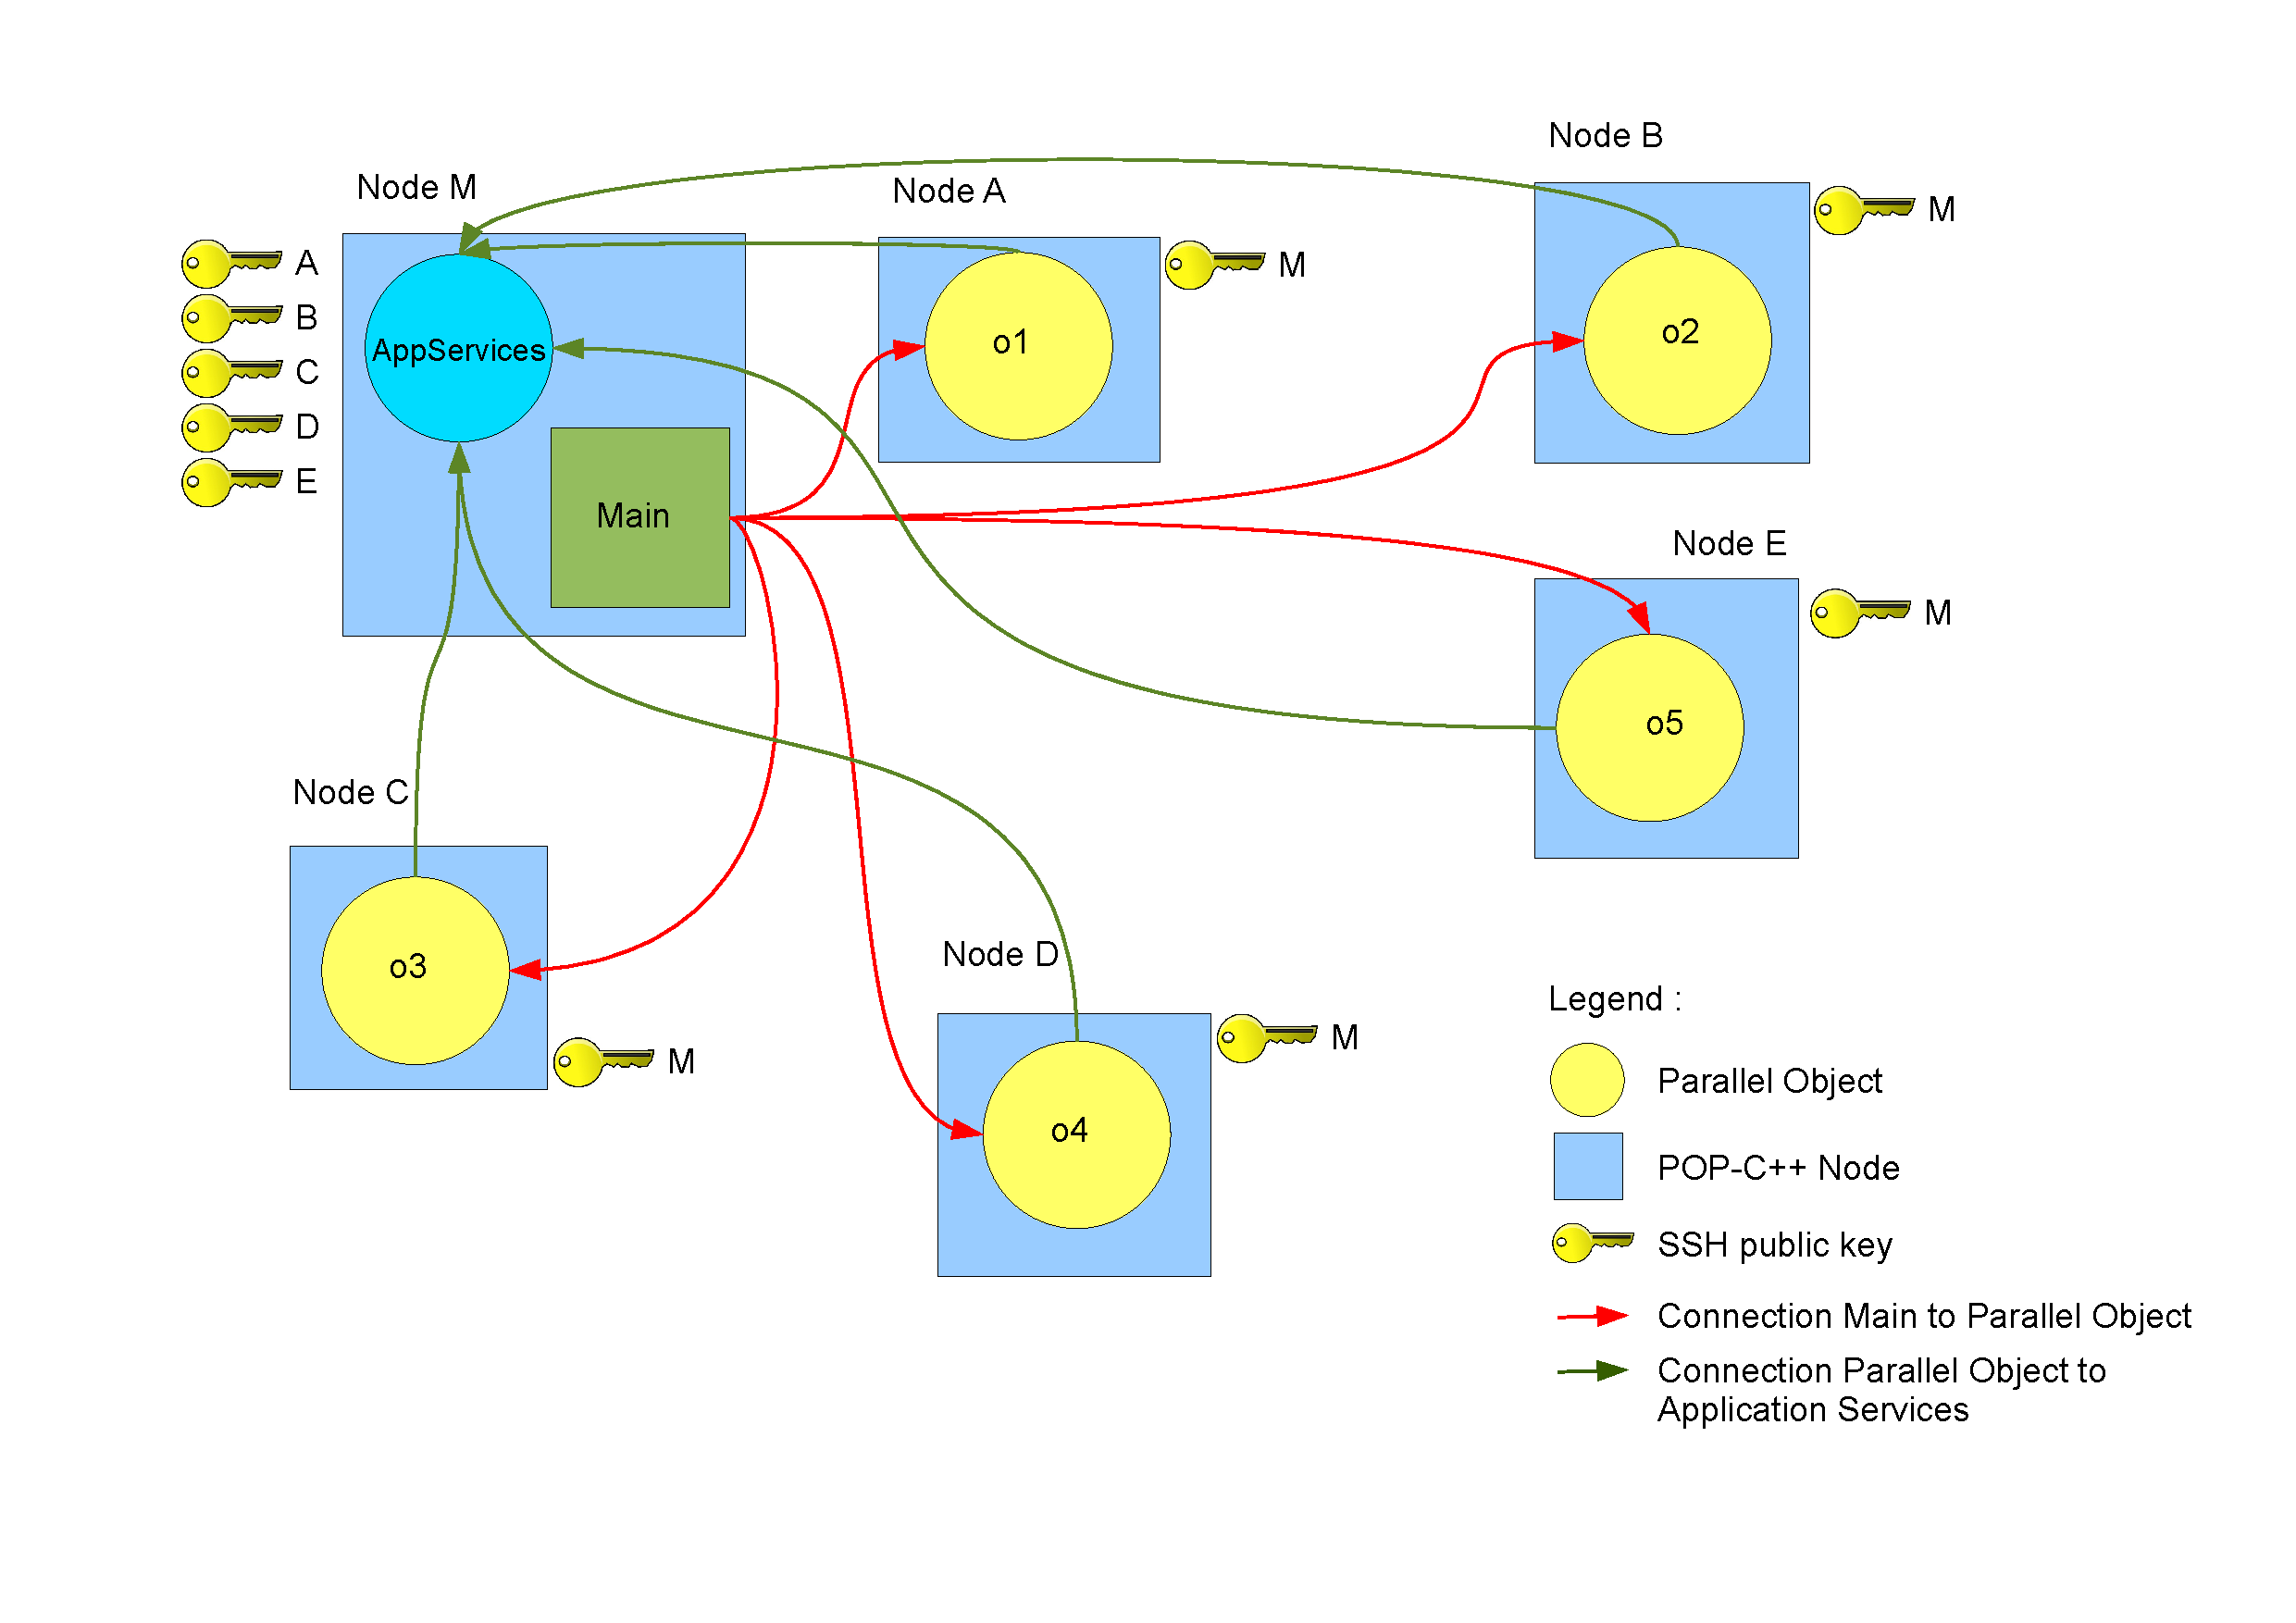
\includegraphics[width=0.70\textwidth]{../main_keys.pdf}
	\label{fig:keys_main}
\end{figure}

The public key of the node running a parallel object is returned to the "Node M" with the resource discovery response. If the response is used to create a parallel object on this specific resource, the public key included in the response is added to the "authorized\_keys" file of the "Node M".\s

This mechanism works in most case where the parallel objects are created only by the "Node M". However, some parallel objects can be created by other parallel objects. In this case, the JobMgr running on the same node as the interface of the object used to create another parallel object will be used to do the resources discovery. In this specific case, we need a mechanism to reroute the PKI included in the response to the "Node M".\s

Figure \ref{fig:ap_mapping} shows the mapping mechanism implemented in POP-C++. When a resource discovery request is propagated by the "Node M" (at least one resource discovery request is initiated by the "Node M"), the access point of the PSM running on the "Node M" is added to the request together with the "Node M" PKI and the POPAppID. When another node receives this request, it will register a mapping between the POPAppID and the PSM access point and another mapping between the POPAppID and the "Node M" PKI. \s

\begin{figure}[ht]
	\caption{POPAppID-AP and POPAppID-PKI Mapping}
  	\centering
	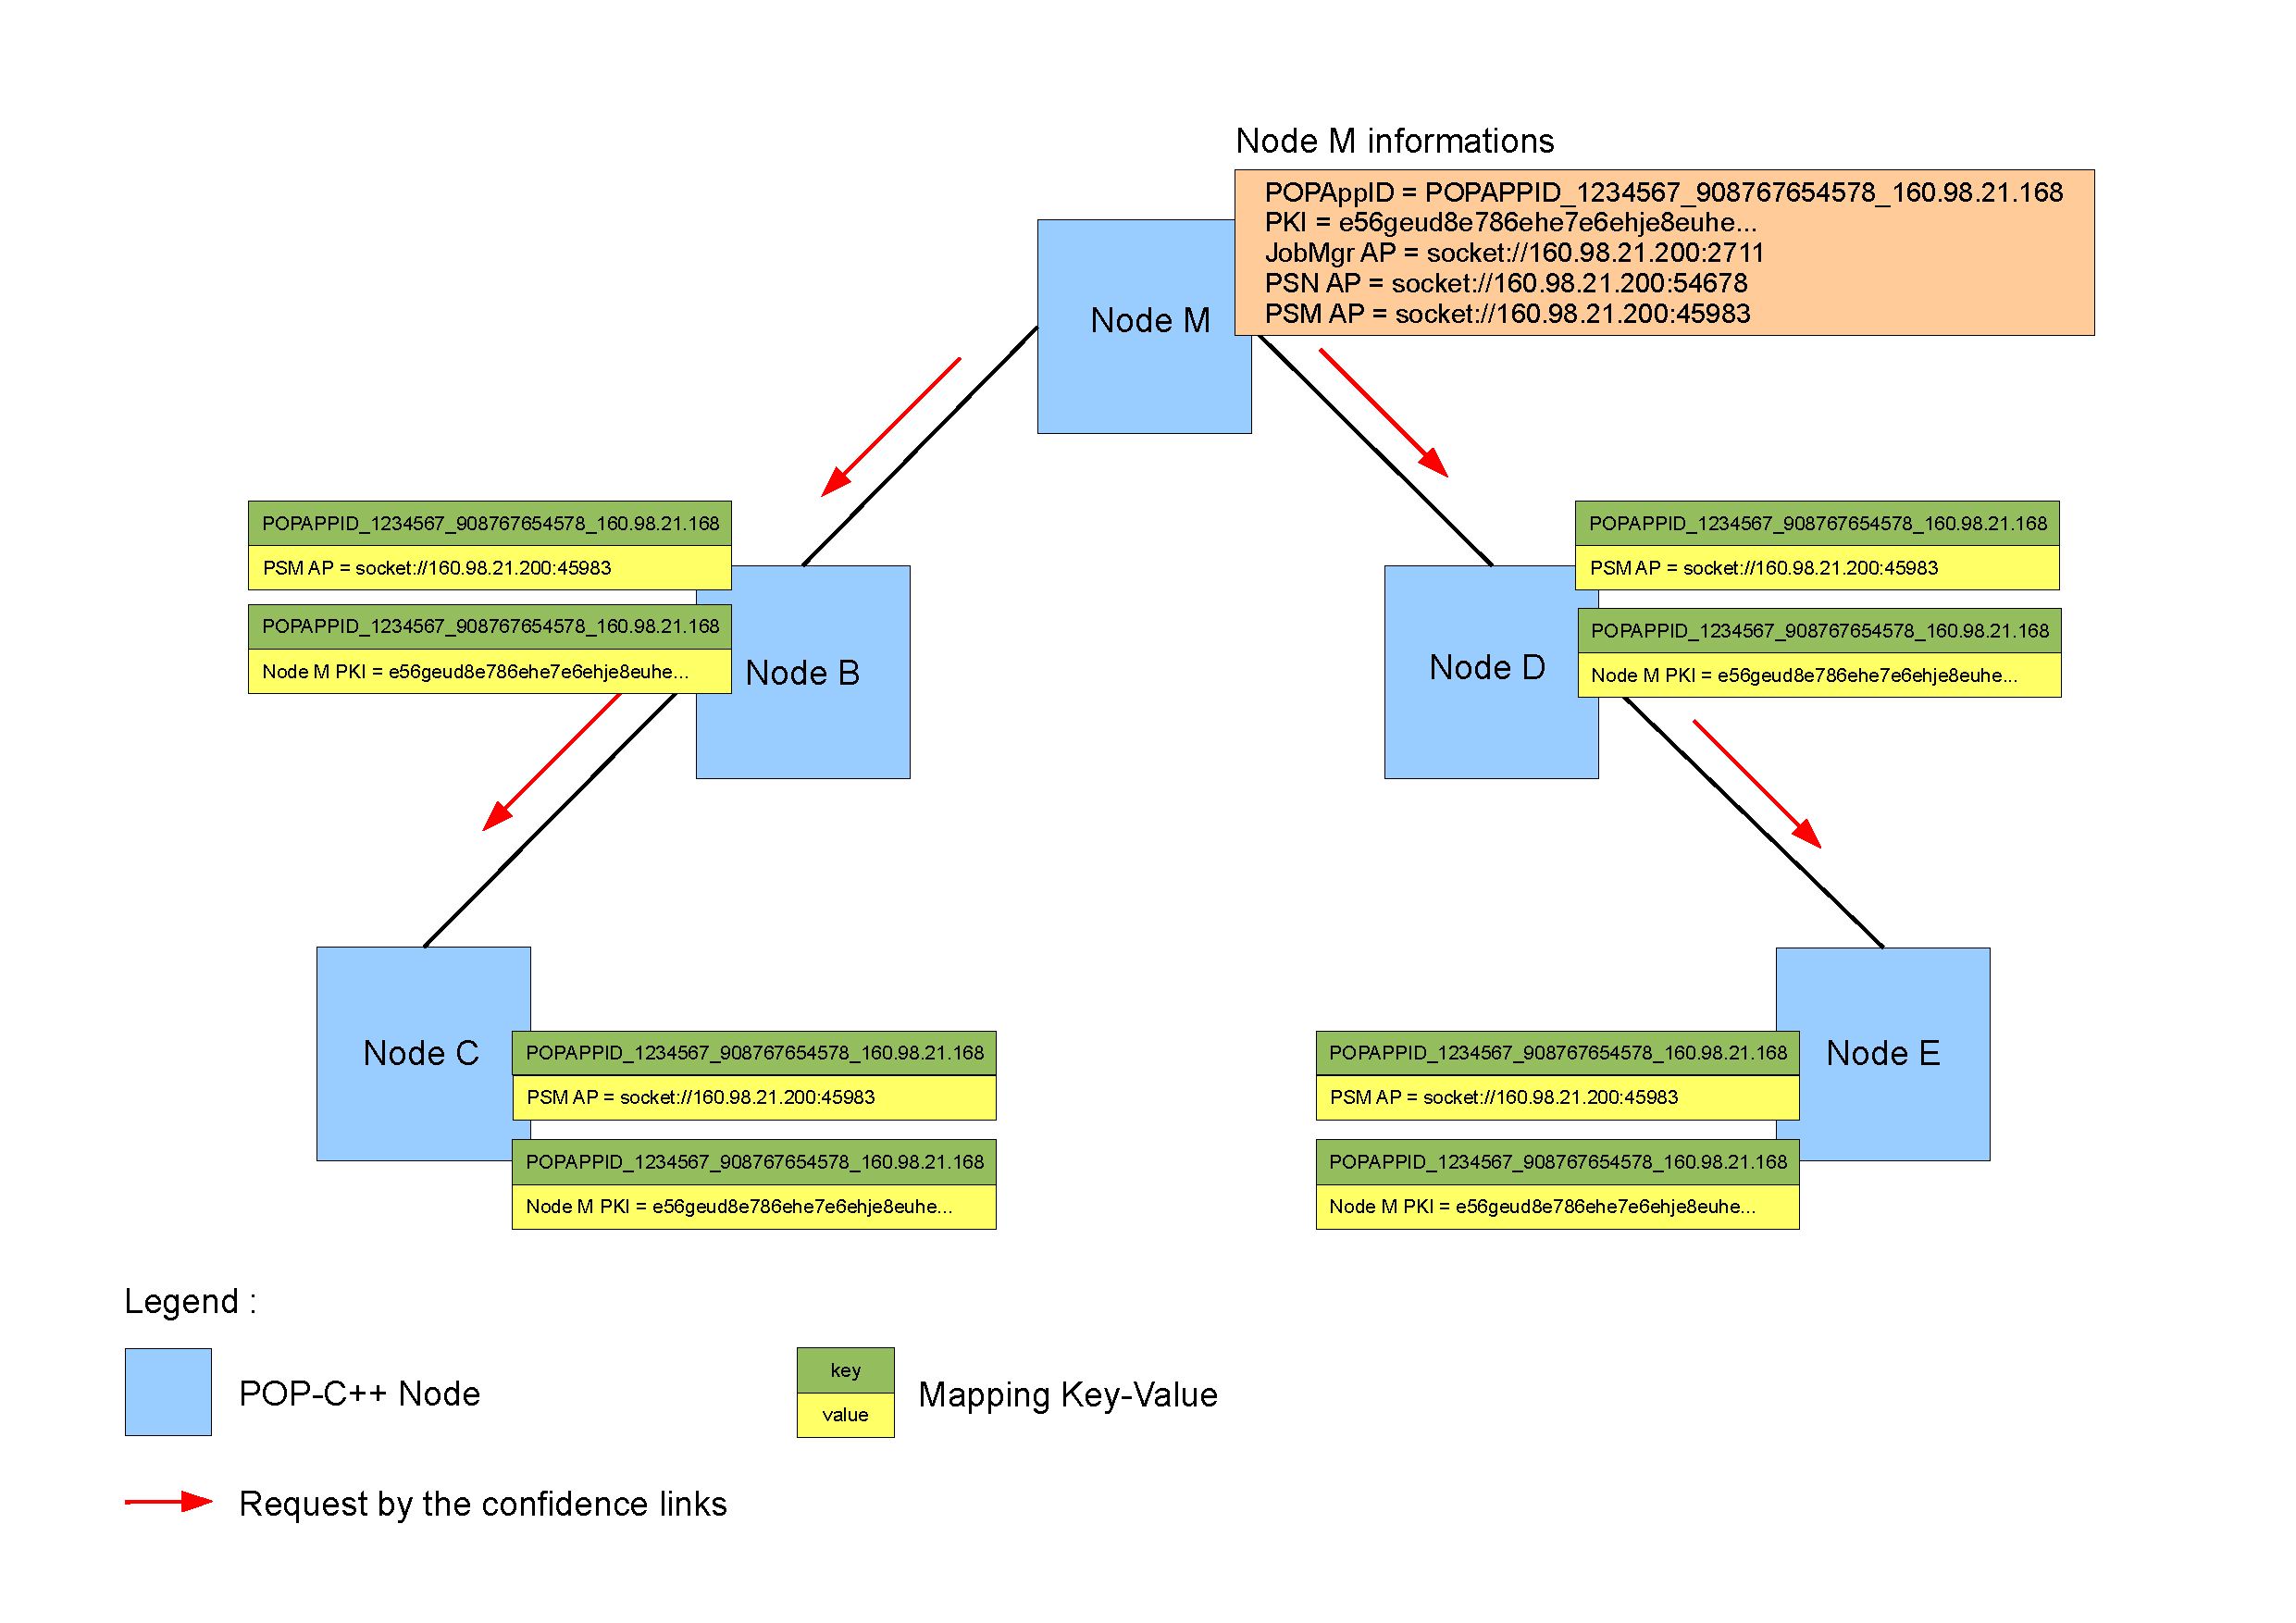
\includegraphics[width=1.0\textwidth]{../ap_mapping.pdf}
	\label{fig:ap_mapping}
\end{figure}


When a resource discovery is initiated by another node than the Node M (in Figure \ref{fig:ap_mapping} Node B-C-D-E), the PKI of Node M will be retrieved in the mapping and added to the request. There are now two different PKI in the request : the PKI of the Node M and the PKI of the Node initiating the resource discovery. When a another Node in the GRID receives this request, it will add the two PKI in its "authorized\_keys" file and send a response if it can execute the request.\s

The initiator Node will receive the response including the PKI of Nodes. These PKI will be redirected to the Node M with the AP-POPAppID mapping.


\subsection{Reference passing}
In this section, we will first discuss the standard process of reference passing inside POP-C++ and then discuss the key exchange in the secure version.

\subsubsection{Reference passing in POP-C++}
A reference of a POP-C++ parallel object is in fact an interface. The interface object can be passed to another parallel object because it inherits from POPBase. The reference passing process in POP-C++ is simply the transfer of an interface object to a parallel object (broker-side). This process is detailed below on each side of the parallel object.\s


\textbf{Interface-side}:
\begin{enumerate}
\item Set the message header in the buffer
\item Serialize the interface into the buffer
\item Send the content of the buffer
\end{enumerate}

\textbf{Broker-side}
\begin{enumerate}
\item Unserialize the interface
\item Cast the interface to the right object (parallel object)
\item Use the interface to make call
\end{enumerate}

\subsubsection{Reference passing and key exchange}

When the reference of an object is passed to another parallel object, some keys must be exchanged as well. In fact, The node running the core of the parallel object (broker-side) must know the public key of the node having the reference of this parallel object. The Interface (the reference of the parallel object) will soon or later contact the Broker. To do that, the Interface will need to create a SSH tunnel to the node executing the Broker.\s

\begin{figure}[ht]
	\caption{Reference Passing}
  	\centering
	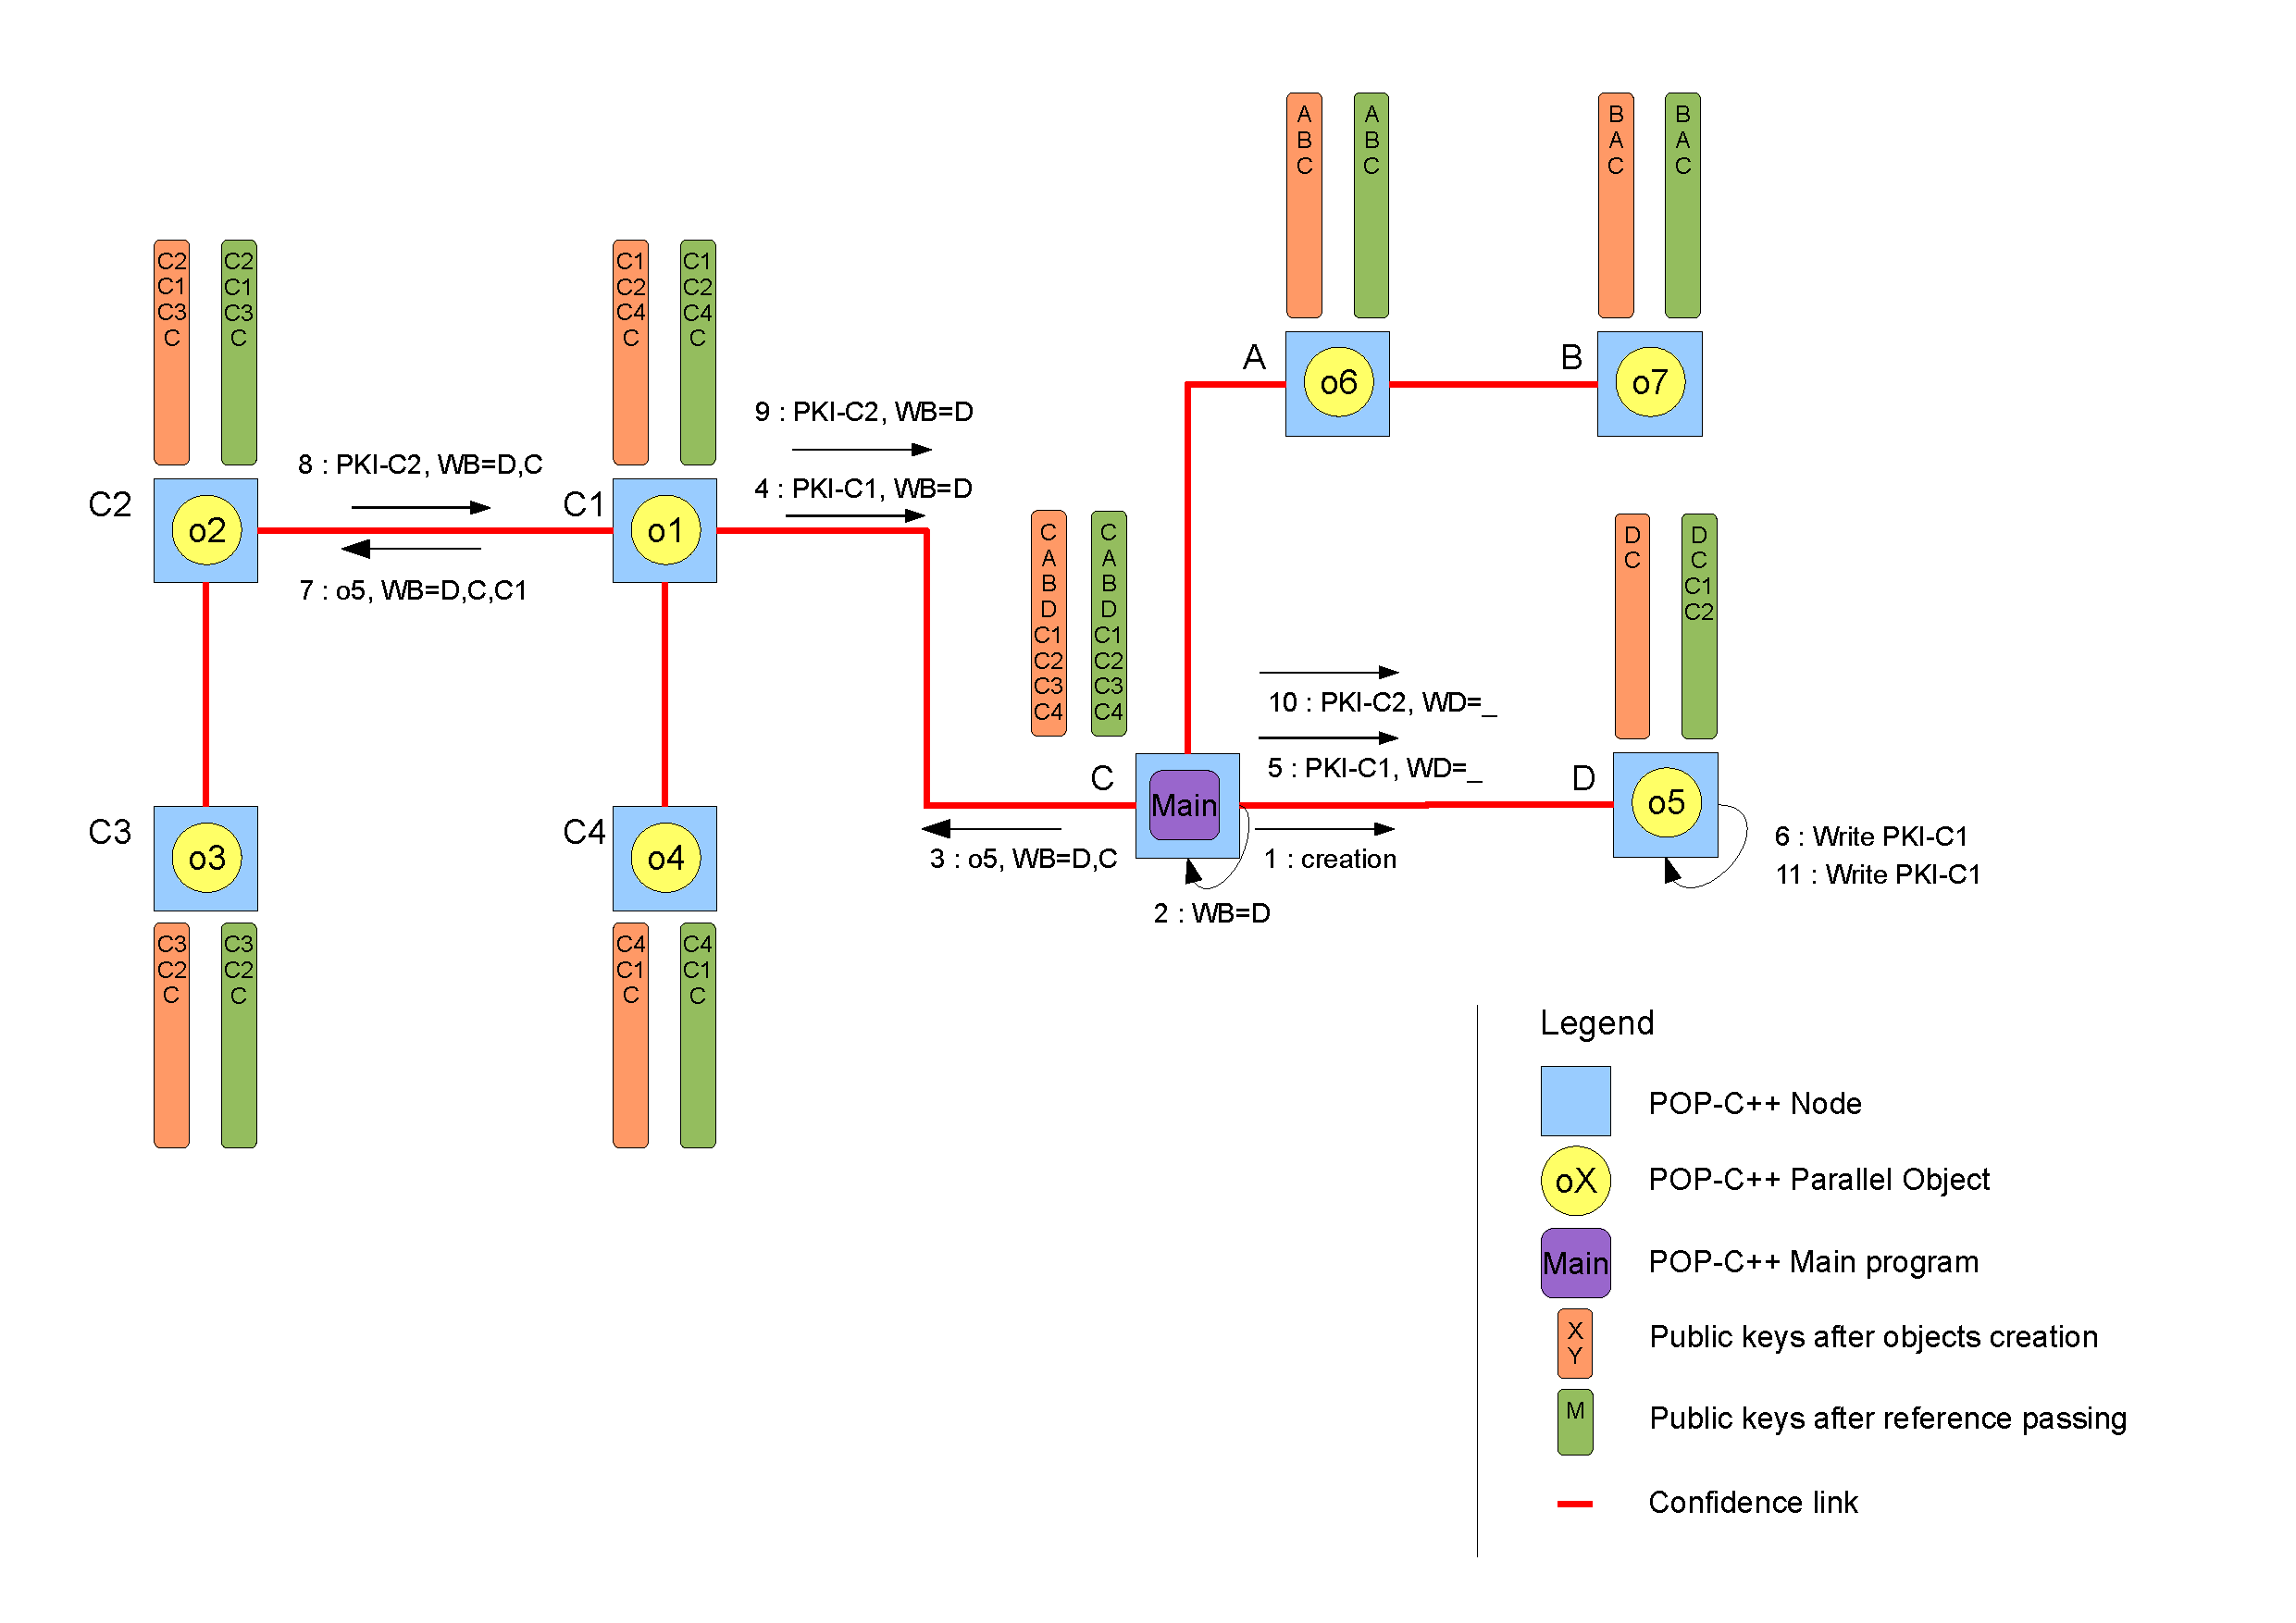
\includegraphics[width=1.0\textwidth]{../ref_passing_impl.pdf}
	\label{fig:ref_passing_impl}
\end{figure}

 As shown in Figure \ref{fig:ref_passing_impl}, the key exchange in during reference passing is going as follows : 

\begin{enumerate}
\item The parallel object "o5" is created by the Node C. The Interface of "o5" is executed on the "Node C". 
\item At its creation, the reference to the node running "o5" ("Node D") has been added to the "POPWayback" object associated with the Interface of "o5". 
\item The reference of the object "o5" is passed to the object "o1". To be passed, the reference will be serialized. During this serialization, the current node of the reference will be added to the "POPWayback" object associated with the reference then it will be sent to the parallel object. 
\item When the object "o1" receives the reference, it will deserialize it. During this deserialization, the PKI of the "Node C1" will be sent to the "Node C". 
\item The "Node C" will reroute this PKI to the "Node D" as stored in the "POPWayback" object. 
\item The "Node D" will write this PKI in its authorized\_keys file.
\item The object "o1" will then send the same reference to the object "o2". The reference will be serialized, the current node ("Node C1" access url) will be added to the "POPWayback" object of the reference and then the reference will be sent.
\item The object "o2" will receive the reference and deserialize it. The PKI of the "Node C2" will be sent to the "Node C1".
\item The "Node C1" will reroute the PKI to the "Node C". 
\item The "Node C" will reroute the PKI to the "Node D".
\item The "Node D" will write this PKI in its authorized\_keys file.
\end{enumerate} 





\subsubsection{Reference passing of Global Services : od.service}
When a reference of a Global Service is passed to another Global Service, the mechanism described above must not be executed. In fact, POP-C++ Global Service only communicates with the initial confidence links. To be able to handle the reference passing of the Global Service, a new object description (od) is introduced to know if a parallel object is a service. This od helps us to know when we are dealing with a service or with a simple parallel class of a POP-C++ application. In case the parallel object is a service, the key exchange for reference passing is disabled. 

This od is added to the three Global Services parallel objects (JobMgr, PSN and PSM). The syntax of this od is : 
\begin{lstlisting}
od.service(bool isService);
\end{lstlisting}


\pagebreak
\subsection{Request and Response by the confidence link}
In POP-C++ 1.3.1 beta, the resource discovery request is propagated by the confidence link in the GRID but the response is sent directly to the initiator Node. To be able to use this resource discovery algorithm in POP-C++ 1.3.1 beta Secure1 (a pre-version of POP-C++ for the ViSaG project), the response needs to be sent to the initiator Node by the confidence link as well. To do this, some modifications have been made. This section is a review of those modifications.

\subsubsection{POPWayback}
\label{lb:popwayback}
The "POPWayback" is an object used to store a path in the GRID. A "POPWayback" object is added to the resource discovery request. A new node is added to this object at each hop in the GRID. When the response must be sent back to the initiator, this object is used to retrieve the path in the GRID and reroute the response by the confidence links. The "POPWayback" object inherits from "POPBase". Due to this, it can be passed between parallel objects.

As shown in Figure \ref{fig:wayback}, a request from the Node A is propagated all over the GRID through the confidence links. In non-secure mode, the answer could be redirected directly to the node A. On the other hand, in secure mode, the response must take the same path that it took to come to the node. The intermediate nodes act as routers for the response.

\begin{figure}[ht]
	\caption{Request - Response in Secure POP-C++}
  	\centering
	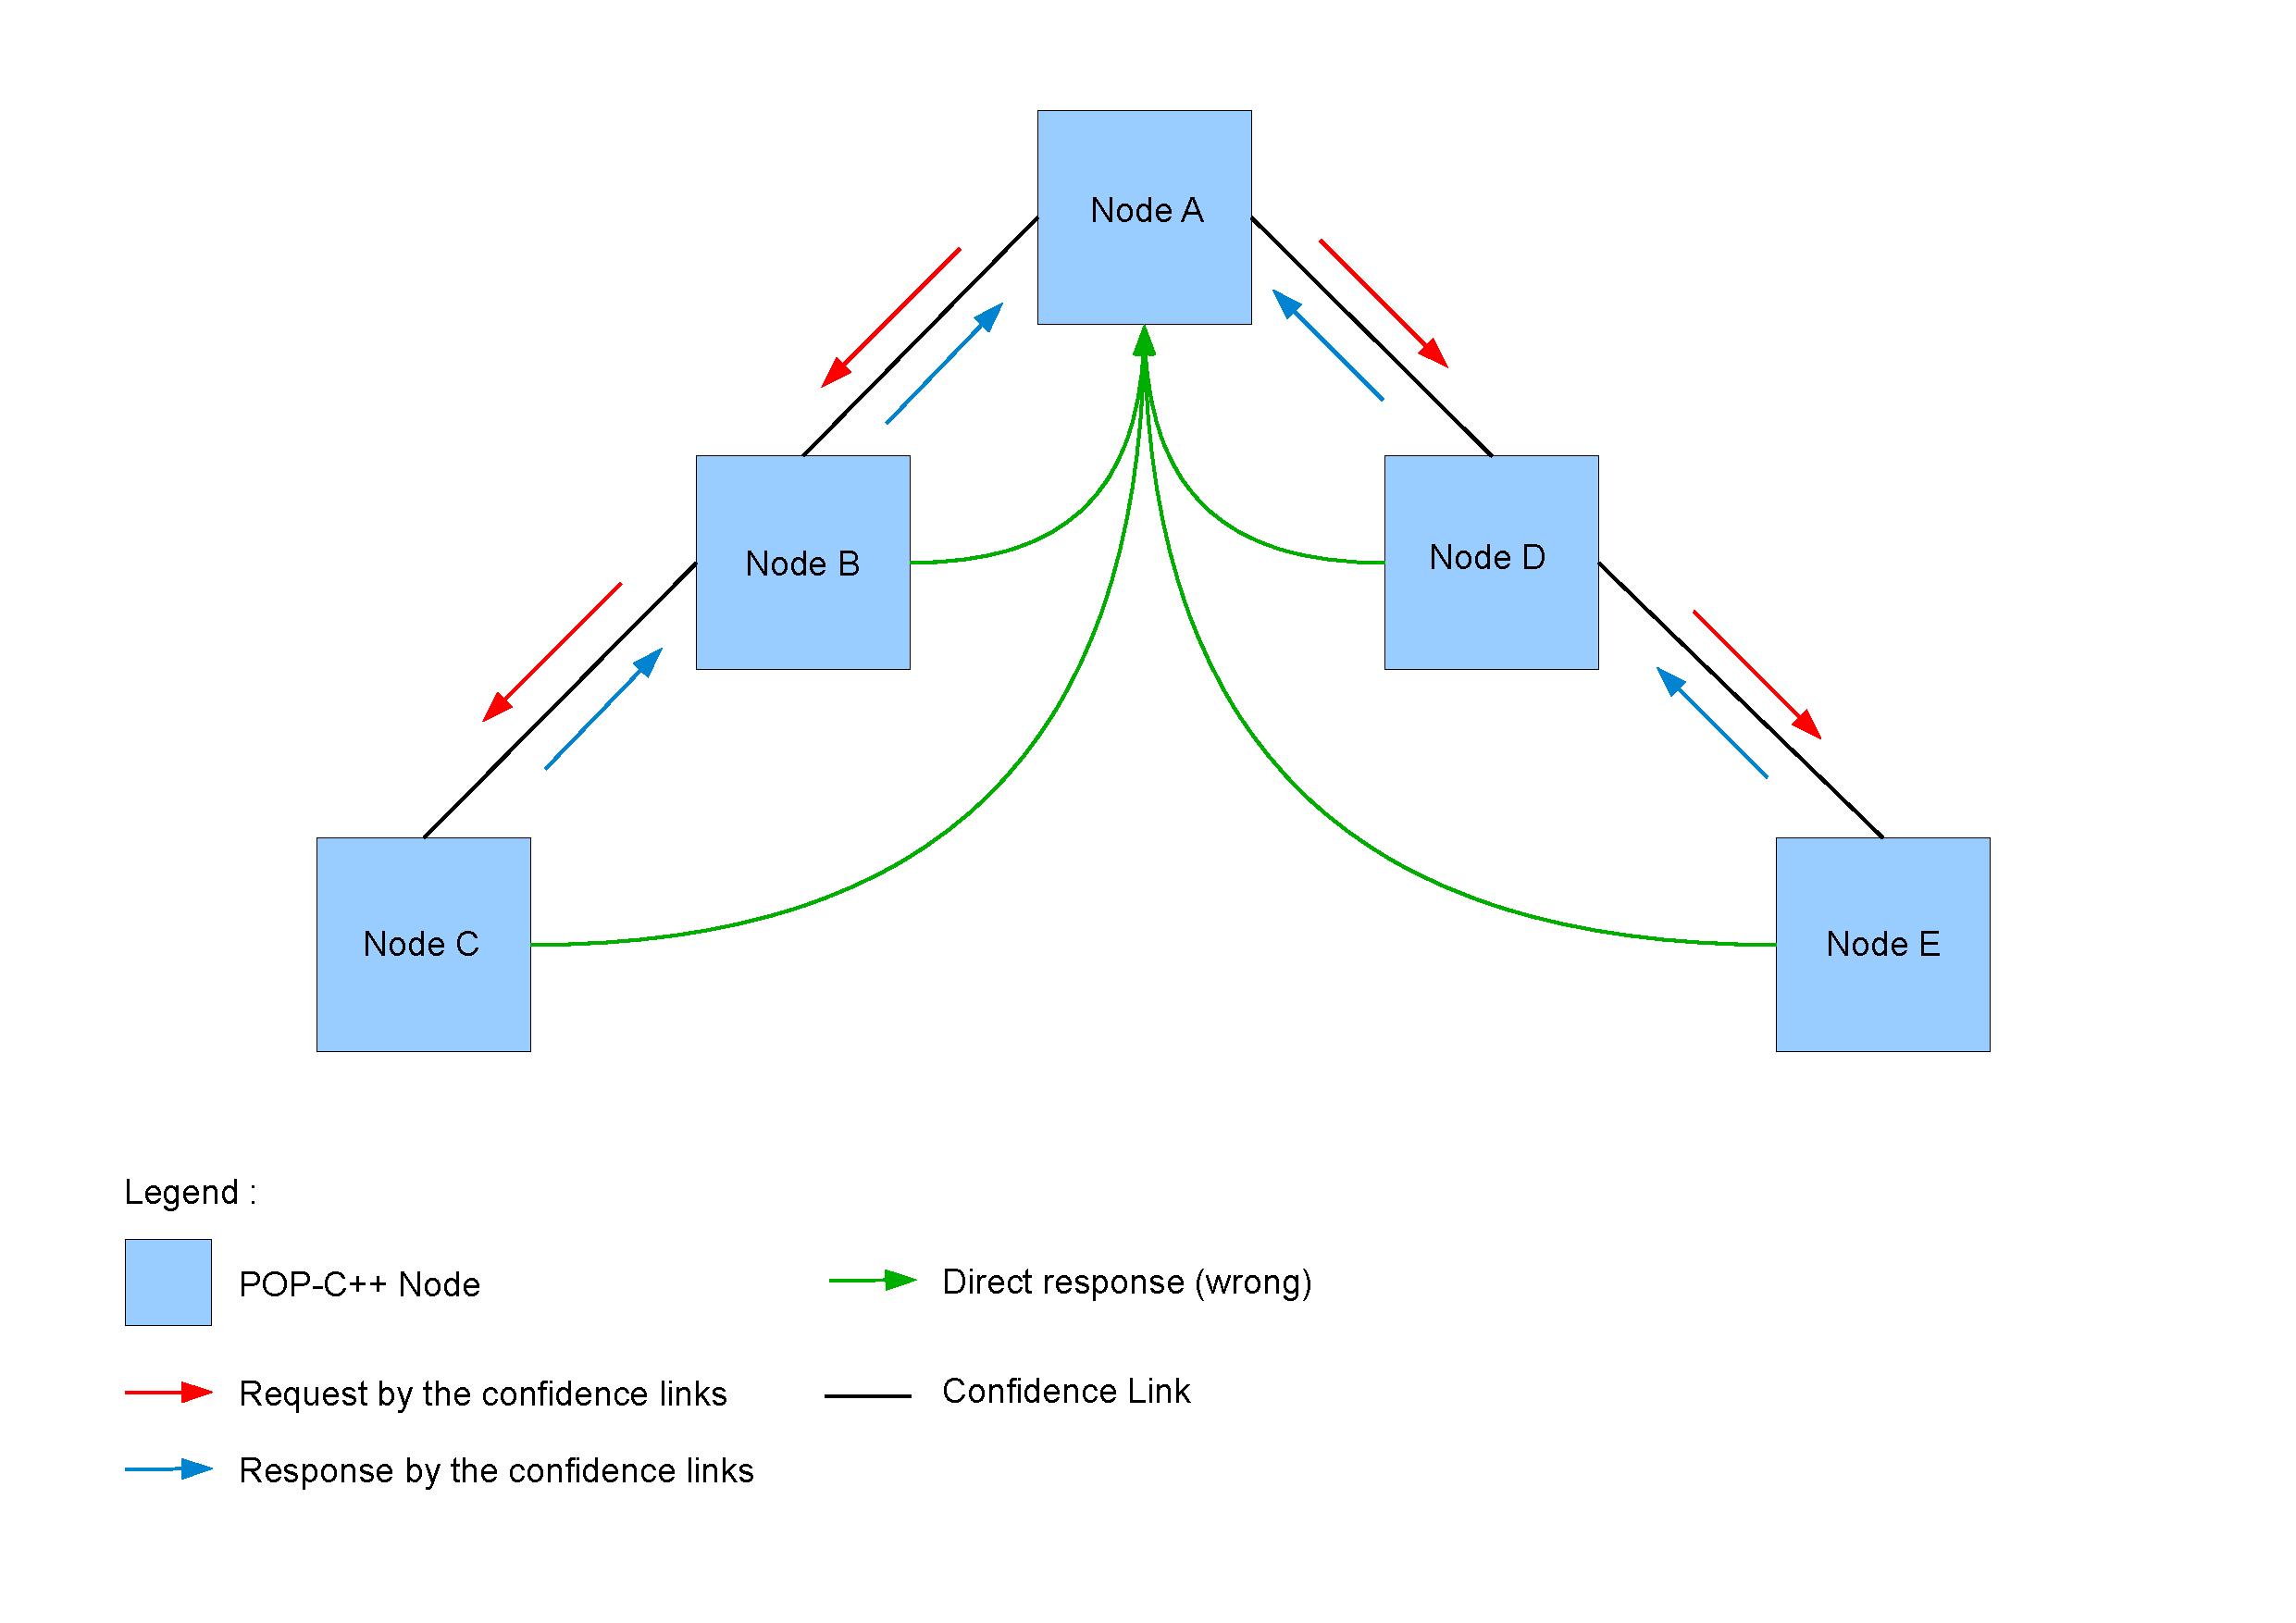
\includegraphics[width=1.0\textwidth]{../wayback.pdf}
	\label{fig:wayback}
\end{figure}

\pagebreak
\section{Future improvements}
In this chapter, the future possible optimizations are explained.

\subsection{Compilation Secure/Non-secure}
At this point, POP-C++ 1.3.1 beta Secure1 is fully secured. It would be a good improvement to let the user choose if he wants to compile a secure version or a non-secure version of POP-C++.

\subsection{Keep authorized\_keys file in memory}
In the current version, an external command is executed to know if a PKI is already in the "authorized\_keys" file. This file should be read at the Global Services start-up and the PKI should be kept in a data structure to avoid the need of an external command.

\subsection{Register SSH tunnel}
In the current implementation, more than one SSH tunnel can be created between two nodes for the same parallel objects. Registering the SSH tunnel created in the PSM could reduce the number of SSH tunnel created between two nodes. 

\subsection{Pseudo-main}
To be fully secure in the virtual world, the main of a POP-C++ application should be a little bit modified to be able to launch the application in a virtual machine as well. This point will be explained more in details later in the document relative to the Virtual version of POP-C++\cite{vpopc_clement}.

\section{Major changes for the user}

\subsection{Overhead}
To be secured, the new version of POP-C++ have to do more job than before. These new tasks may add an overhead on the execution of a POP-C++ application. This overhead is due to two specific points : 

\begin{enumerate}
\item \textbf{New messages: } to exchange the keys between the nodes, some new messages have been added. These new messages are sent when an object is created by a JobMgr other than the JobMgr of the "Main Node" and when a parallel object reference is passed between nodes.
\item \textbf{Tunnel creation: } to secure the connection, the interface has to create a SSH tunnel. This creation may take some time due to the authentication process.
\item \textbf{Encryption/Decryption: } due to the use of SSH, each communication will pass through an encryption process and a decryption process. This two processes could add some overheads.
\end{enumerate}

\subsection{Compatibility}
There is no compatibility between the version 1.3.1 beta Secure1 and the version 1.3. Due to major changes between these two versions, the POP-C++ application compiled with 1.3 must be recompiled with the new version. All the nodes on the GRID must be upgraded to the new version. The gap between 1.3 and 1.3.1 beta is to big to keep the compatibility.

\pagebreak
\section{Test}
This chapter reviews two main tests that have been made to verify the behaviour of the new version of POP-C++.

\subsection{Scenario 1 : Key exchange in parallel objects creation}
The first scenario aims to test the new version of POP-C++ in creation process. When the POP-C++ global services creates the parallel objects, some keys are exchanged.\s

Figure \ref{fig:ke_creation} shows the sequence diagrams of the creation of 4 parallel objects by three different Nodes. The two first objects are created by the first Nodes (the orange Node). In this case, the key exchange is very simple. The PKI of the Main Node is given to the other Node with the resource discovery request. The key of the Node running the parallel object is given back to the main Node with the resource discovery response. \s

As shown on Figure \ref{fig:ke_creation}, the mapping used in the key exchange are added during the first resource discovery launched from the Node A. These mappings are used later by the other nodes for the key exchange.\s

For the two last objects created, the process is slightly different. This time, the second Node (pink Node) is in charge of the object creation. Due to that, the key of the nodes running the parallel object must be redirected to the main Node. \s

The majority of the process is identical to the first two creation. When the key is returned with the resource discovery response, the Node in charge of the object creation (pink Node) will redirect the key to the Main Node (orange Node). \s

At the end of the creation process, every node will have the PKI of the Node A. The Node A (the Main Node) will have the key of every nodes running a parallel object of the application.\s

The application used to test this behaviour is "multiobj" which is available in the source of POP-C++. The test has been made with five nodes running one parallel objects. The application run successfully, and the "authorized\_keys" file of each nodes were as expected. 

\begin{figure}[ht]
	\caption{Scenario 1 : Key exchange in parallel objects creation}
  	\centering
	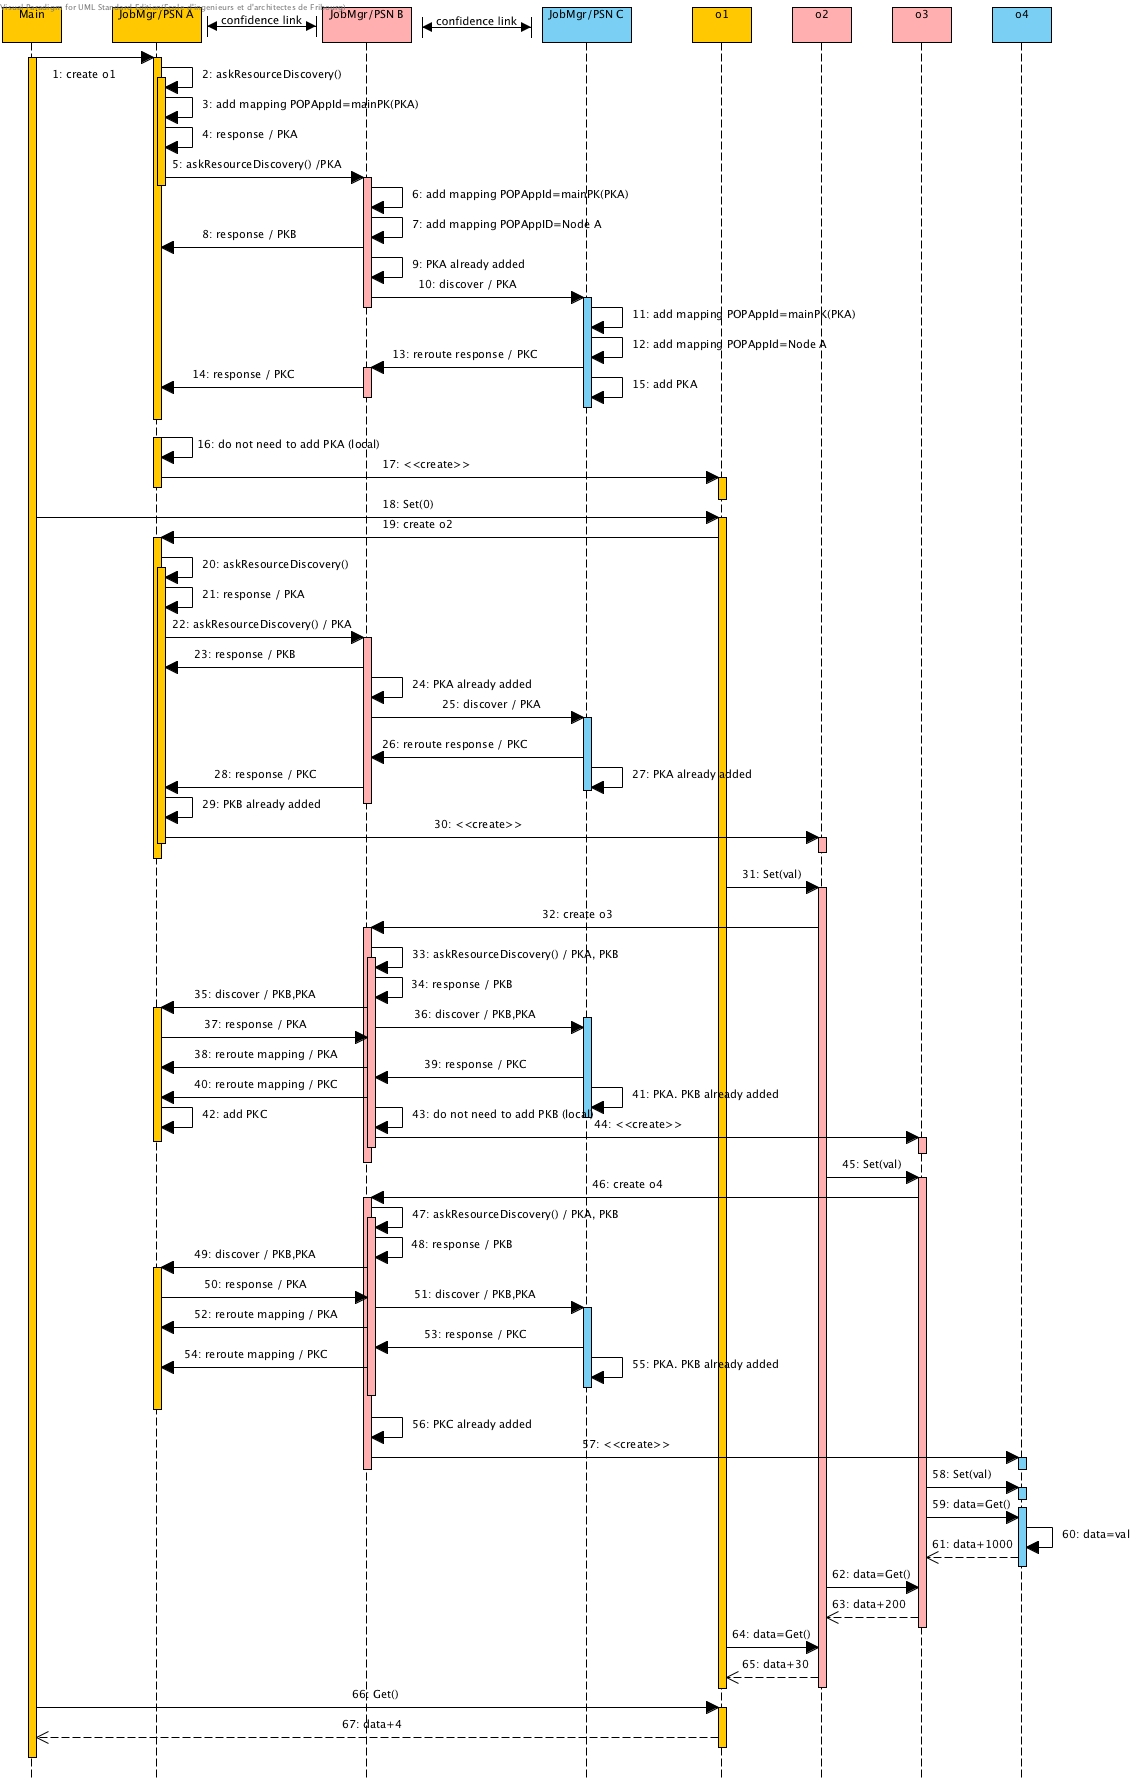
\includegraphics[scale=0.35]{../ke_creation.jpg}
	\label{fig:ke_creation}
\end{figure}
\clearpage

\subsection{Scenario 2 : Key exchange in reference passing}
The second scenario aims to test the new POP-C++ version in the reference passing process. When the main program or a parallel object pass a parallel object reference to another parallel object, the node running the parallel object pointed by the reference must receive the public key of the node receiving the reference.\s

Figure \ref{fig:ke_refpassing} shows the "demopopc" program running on three different nodes. The nodes B and C are connected to the node A (confidence link). The nodes B and C are not connected to each other. \s

The main program send the reference of "o2" to "o1". On the deserialization of the reference of "o2" on "o1", the PSM A will be contacted and the PKI will be redirected to the Node B. On the Node B, the key will be added.\s

The main program send the reference of "o3" to "o2". On the deserialization of the reference of "o3" on "o2", the PSM B will be contacted and the PKI will be redirected to the Node A and to the Node C. On the Node C, the key will be added.\s

The main program send the reference of "o1" to "o3". On the deserialization of the reference of "o1" on "o3", the PSM C will be contacted and the PKI will be redirected to the Node A. On the Node A, the key will be added.\s


\begin{figure}[!ht]
	\caption{Scenario 2 : Key exchange in reference passing}
  	\centering
	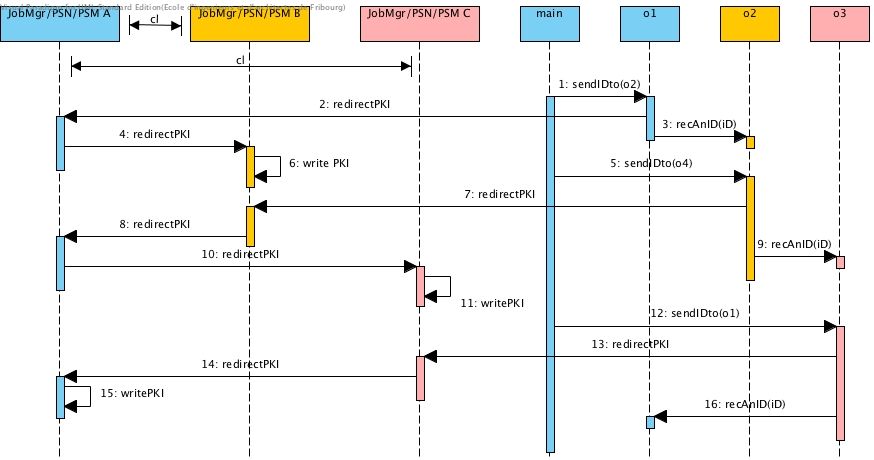
\includegraphics[width=1.0\textwidth]{../ke_refpassing.jpg}
	\label{fig:ke_refpassing}
\end{figure}

The application used to test this behaviour is "demopopc" which is available in the source of POP-C++. The test has been made with three nodes running one parallel objects. The application run successfully, and the "authorized\_keys" file of each nodes were as expected. 

\pagebreak
\subsection{Code improvements}
This section explains some tools that have been used to improve the code of POP-C++ 1.3.1 beta secure 1.

\subsubsection{Warnings check}
The whole code have been compiled with the full warning check from the C++ compiler. The majority of the warnings have been remove. Please check Chapter \ref{known_issues} on Page \pageref{known_issues} to know which warnings are still on the current code. \s

To compile the POP-C++ with all warnings on, the configure script must received some additional options. The code used is presented below : \s

\begin{lstlisting}
./configure CPPFLAGS=-Wall --prefix=/home/visag/popc
\end{lstlisting}

\subsubsection{Memory allocation check}
The memory allocation and deallocation have been checked with the MALLOC\_CHECK\_ environment variable. If this variable is set to 1, the "malloc()" call used a different implementation (with less performance) that is able to output any diagnostic on stderr.\s

To run the Global Services with the MALLOC\_CHECK\_ variable, use the following command : 
\begin{lstlisting}
MALLOC_CHECK_=1 SXXpopc start
\end{lstlisting}\s

Use the same to launch the POP-C++ application
\begin{lstlisting}
MALLOC_CHECK_=1 popcrun obj.map ./main ...
\end{lstlisting}\s

This test has not revealed any allocation problem in POP-C++. \s

It's planned to try to use "valgrind"\cite{valgrind} to have a better check of any memory leaks and bugs. For the moment, this tools has not been used in the current version. It would be great to use it in the final version of POP-C++ for the ViSaG project. 

\pagebreak
\section{Known issues}
\label{known_issues}
\subsection{Latency on SSH authentication}
Sometimes, the authentication to create a SSH tunnel takes more time than expected. This phenomenon has not been explained yet. A discussion with SSH expert must be hold.

\subsection{Remaining warnings}
There are still some remaining warnings in the current compilation of POP-C++ 1.3.1 beta secure 1. These warnings are explained below : \s

\textbf{AppCoreService constructor warning} : This warning is due to a different declaration of the constructor in the header file and in the .cc file. Actually, the header file does not declare "paroc\_service\_base" as a class inherited by "AppCoreService" but in the .cc file, this class is initialized before the other classes declared.\s

\textbf{Warnings in the compiler} : The classes belonging to the compiler have not been modified yet to remove the warnings but they could be easily removed.\s



\section{Conclusion}
POP-C++ 1.3.1 beta Secure1, is a functional version of POP-C++ implementing the security with the SSH tunnelling function. Some future optimizations can be made but there are not vitals for the current project. They will be done if we have the time. POP-C++ 1.3.1 beta Secure1 is a need for the ViSaG project.






\pagebreak





\section{Table of figures}
\listoffigures{}

\section{References}
\begin{thebibliography}{9}

\bibitem{ssh}
	IETF,
  	\emph{SSH : Secure Shell (rfc 4251)}.
	Network Working Group, http://www.ietf.org/rfc/rfc4251.txt
	January 2006.
	
\bibitem{vpopc_clement}
	Valentin Clément,
  	\emph{Virtual POP-C++ : road to ViSaG}. GRID and Cloud Computing Group, EIA-FR, Switzerland, November 2010.
  	
\bibitem{valgrind}
	Valgrind Developers,
  	\emph{Valgrind}. http://valgrind.org

\end{thebibliography}


\end{document}
